\documentclass[a4paper,fontsize=9.0pt]{scrartcl}
\usepackage{float}
% \usepackage[10pt]{extsizes}
\usepackage[utf8]{inputenc}
\usepackage[margin=0.9in]{geometry}
\usepackage{titling}
\usepackage{graphicx}
\graphicspath{ {./Graphs/} }
\setlength{\droptitle}{-5em}

\title{\textbf{Baselines - Combating Partisan Homogenization in News Recommendation Systems}}
\date{\vspace{-10ex}}
\begin{document}
\maketitle

\tableofcontents

\newpage
\section{General Experiment Settings}
\textbf{github-url} : https://github.com/karthikshivaram24/Combatting-partisan-homogenization
\begin{flushleft}
\begin{itemize}
  \item News Articles Used : \textbf{127344}
  \item Features: \textbf{TF-IDF}
  \item Dimensionality Reduction : \textbf{SVD}
  \item Clustering Algorithm : \textbf{K-Means}
  \item Number of Clusters : \textbf{1000}
  \item Cluster Pair Filtering 
  \begin{itemize}
      \item Minimum Cluster Size : \textbf{500}
      \item Minimum Partisan Size : \textbf{0.5}(used balanced sampling to make label distributions equal)
  \end{itemize}
  \item Recommendation Model
  \begin{itemize}
      \item Logistic Regression
      \item SGDClassifier with log loss
  \end{itemize}
  \item Performance Metrics
  \begin{itemize}
      \item \textbf{Macro} : F1, precision , recall
      \item \textbf{@K} : F1, precision, recall
  \end{itemize}
  \item User Preferences:
  \begin{itemize}
      \item \textbf{Homogeneous} : Likes articles of the same partisan score across cluster pair ( Likes conservative articles in both clusters)
      \item \textbf{Heterogeneous} : Likes articles of different partisan score across cluster pair (Likes conservative articles in cluster 1 and liberal articles in cluster 2)
  \end{itemize}
\end{itemize}
\begin{figure}[H]
 \centering
 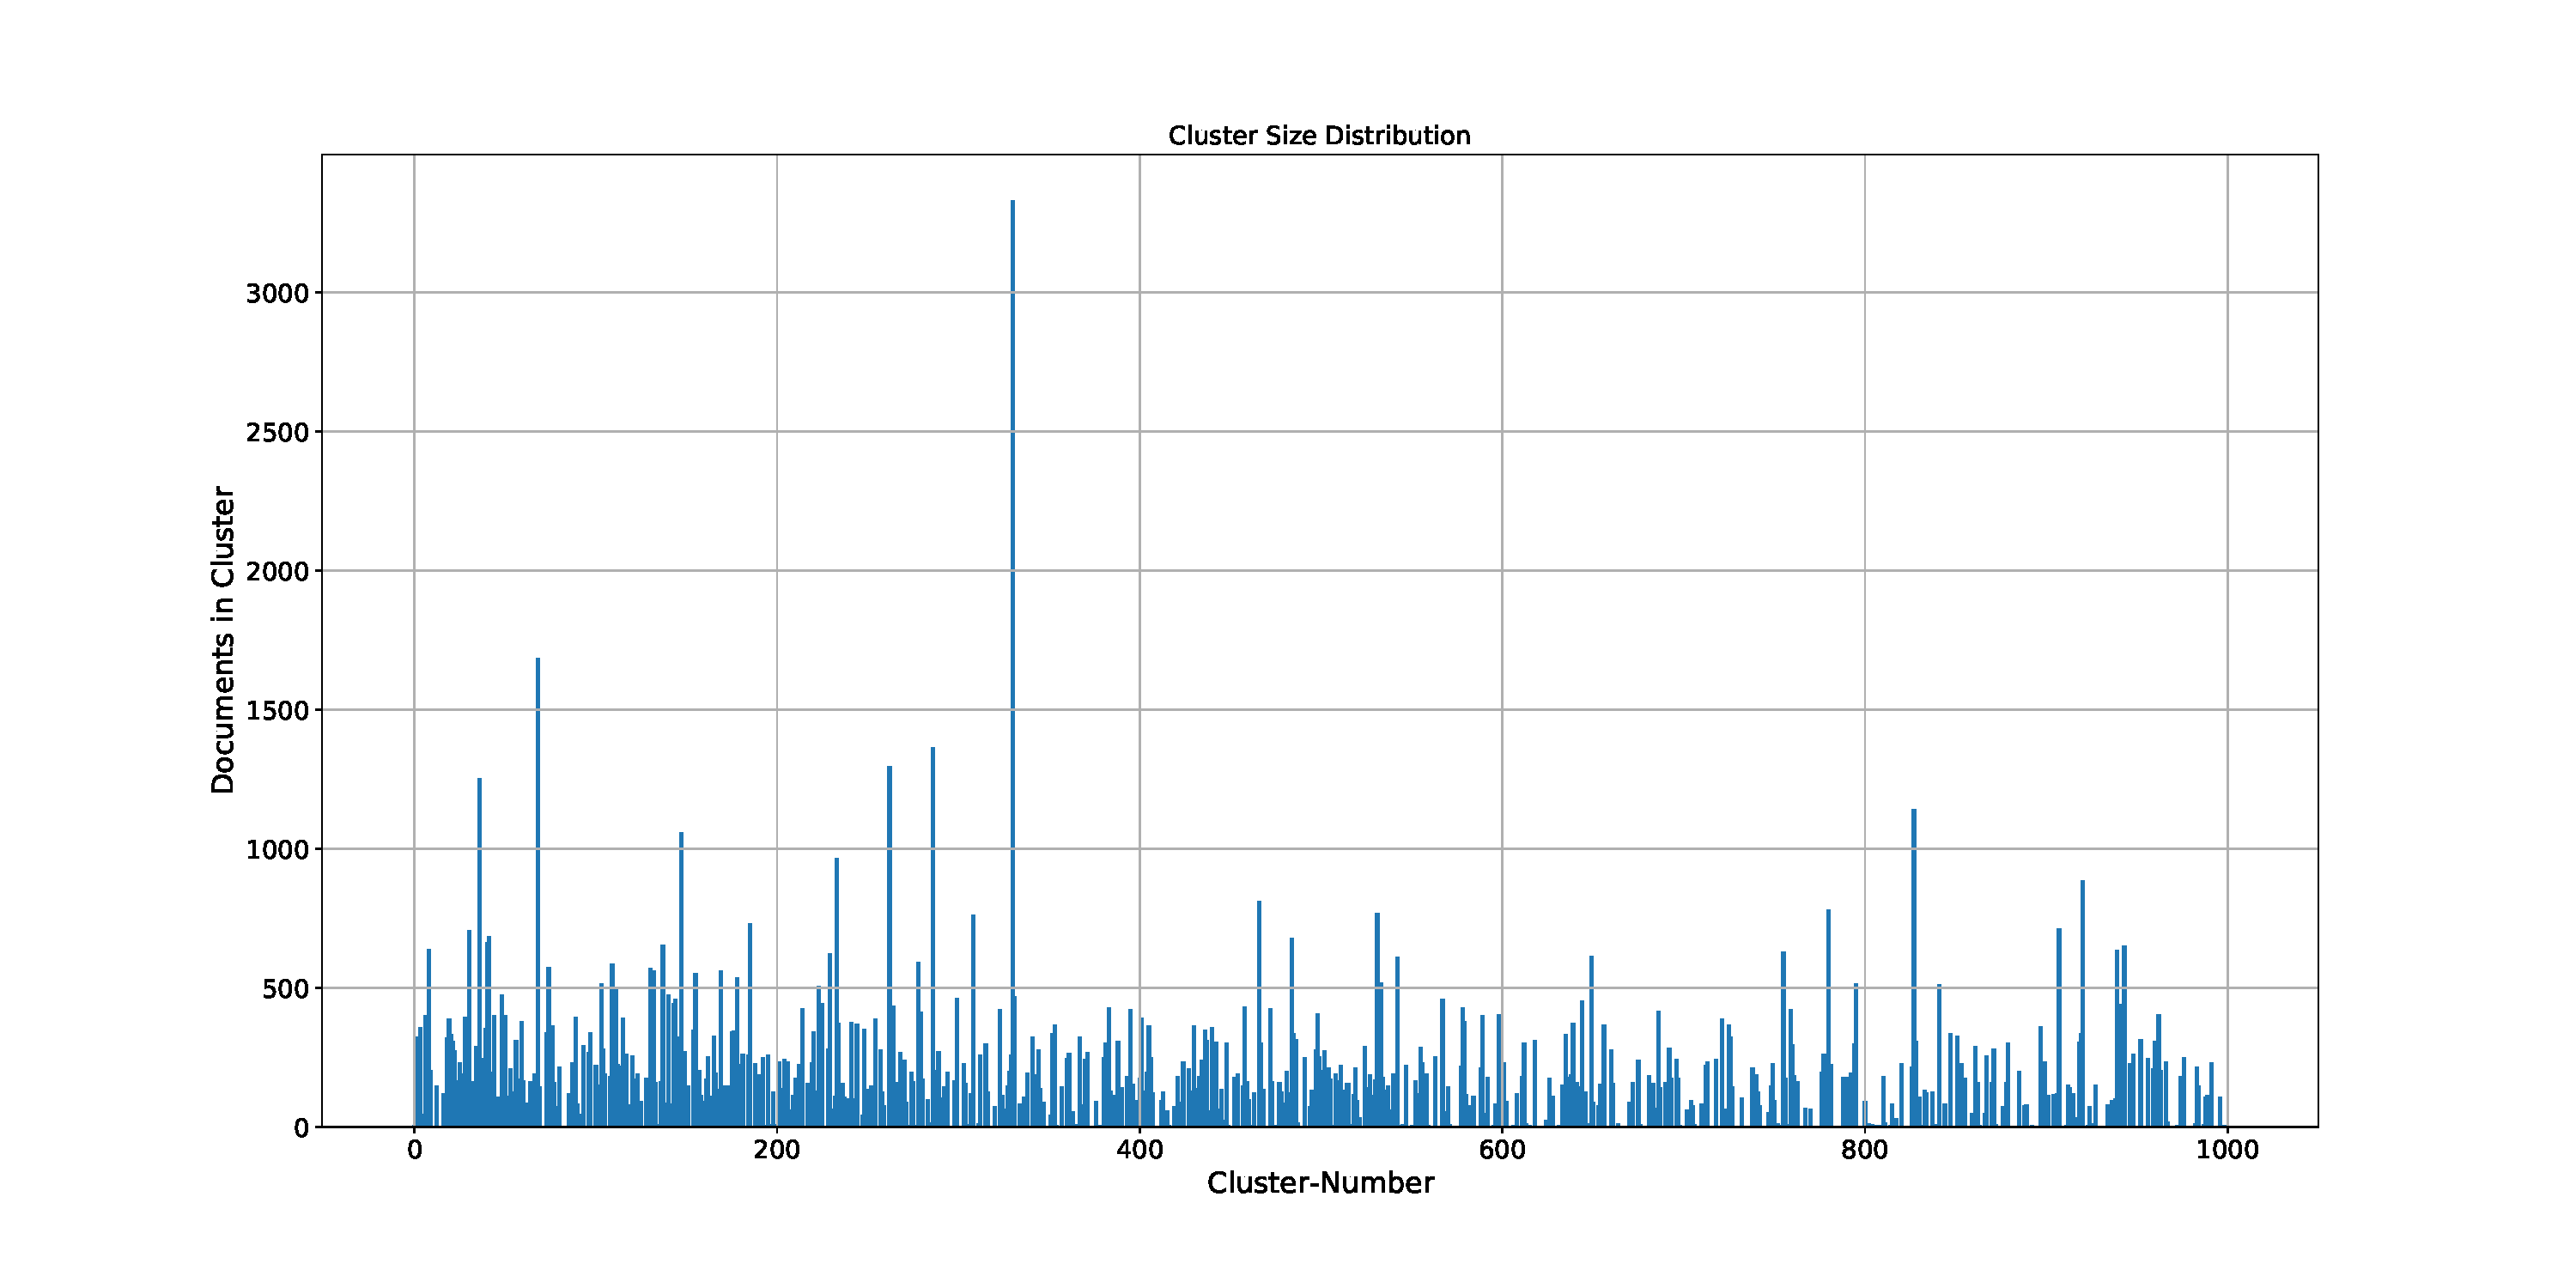
\includegraphics[width=1.0\textwidth]{Graphs/cluster_size_dist.pdf}
\end{figure}
\end{flushleft}


\newpage
\section{Baseline 1: How Topic Similarity affects Model Performance}
\begin{flushleft}
Here we want to measure how well a recommendation system performs on an unseen topic for users with different types of preferences and how this performance varies as similarity between topics increases (seen and unseen topic similarity).
\end{flushleft}
\vspace{-5ex}
\begin{figure}[H]
%  \centering
 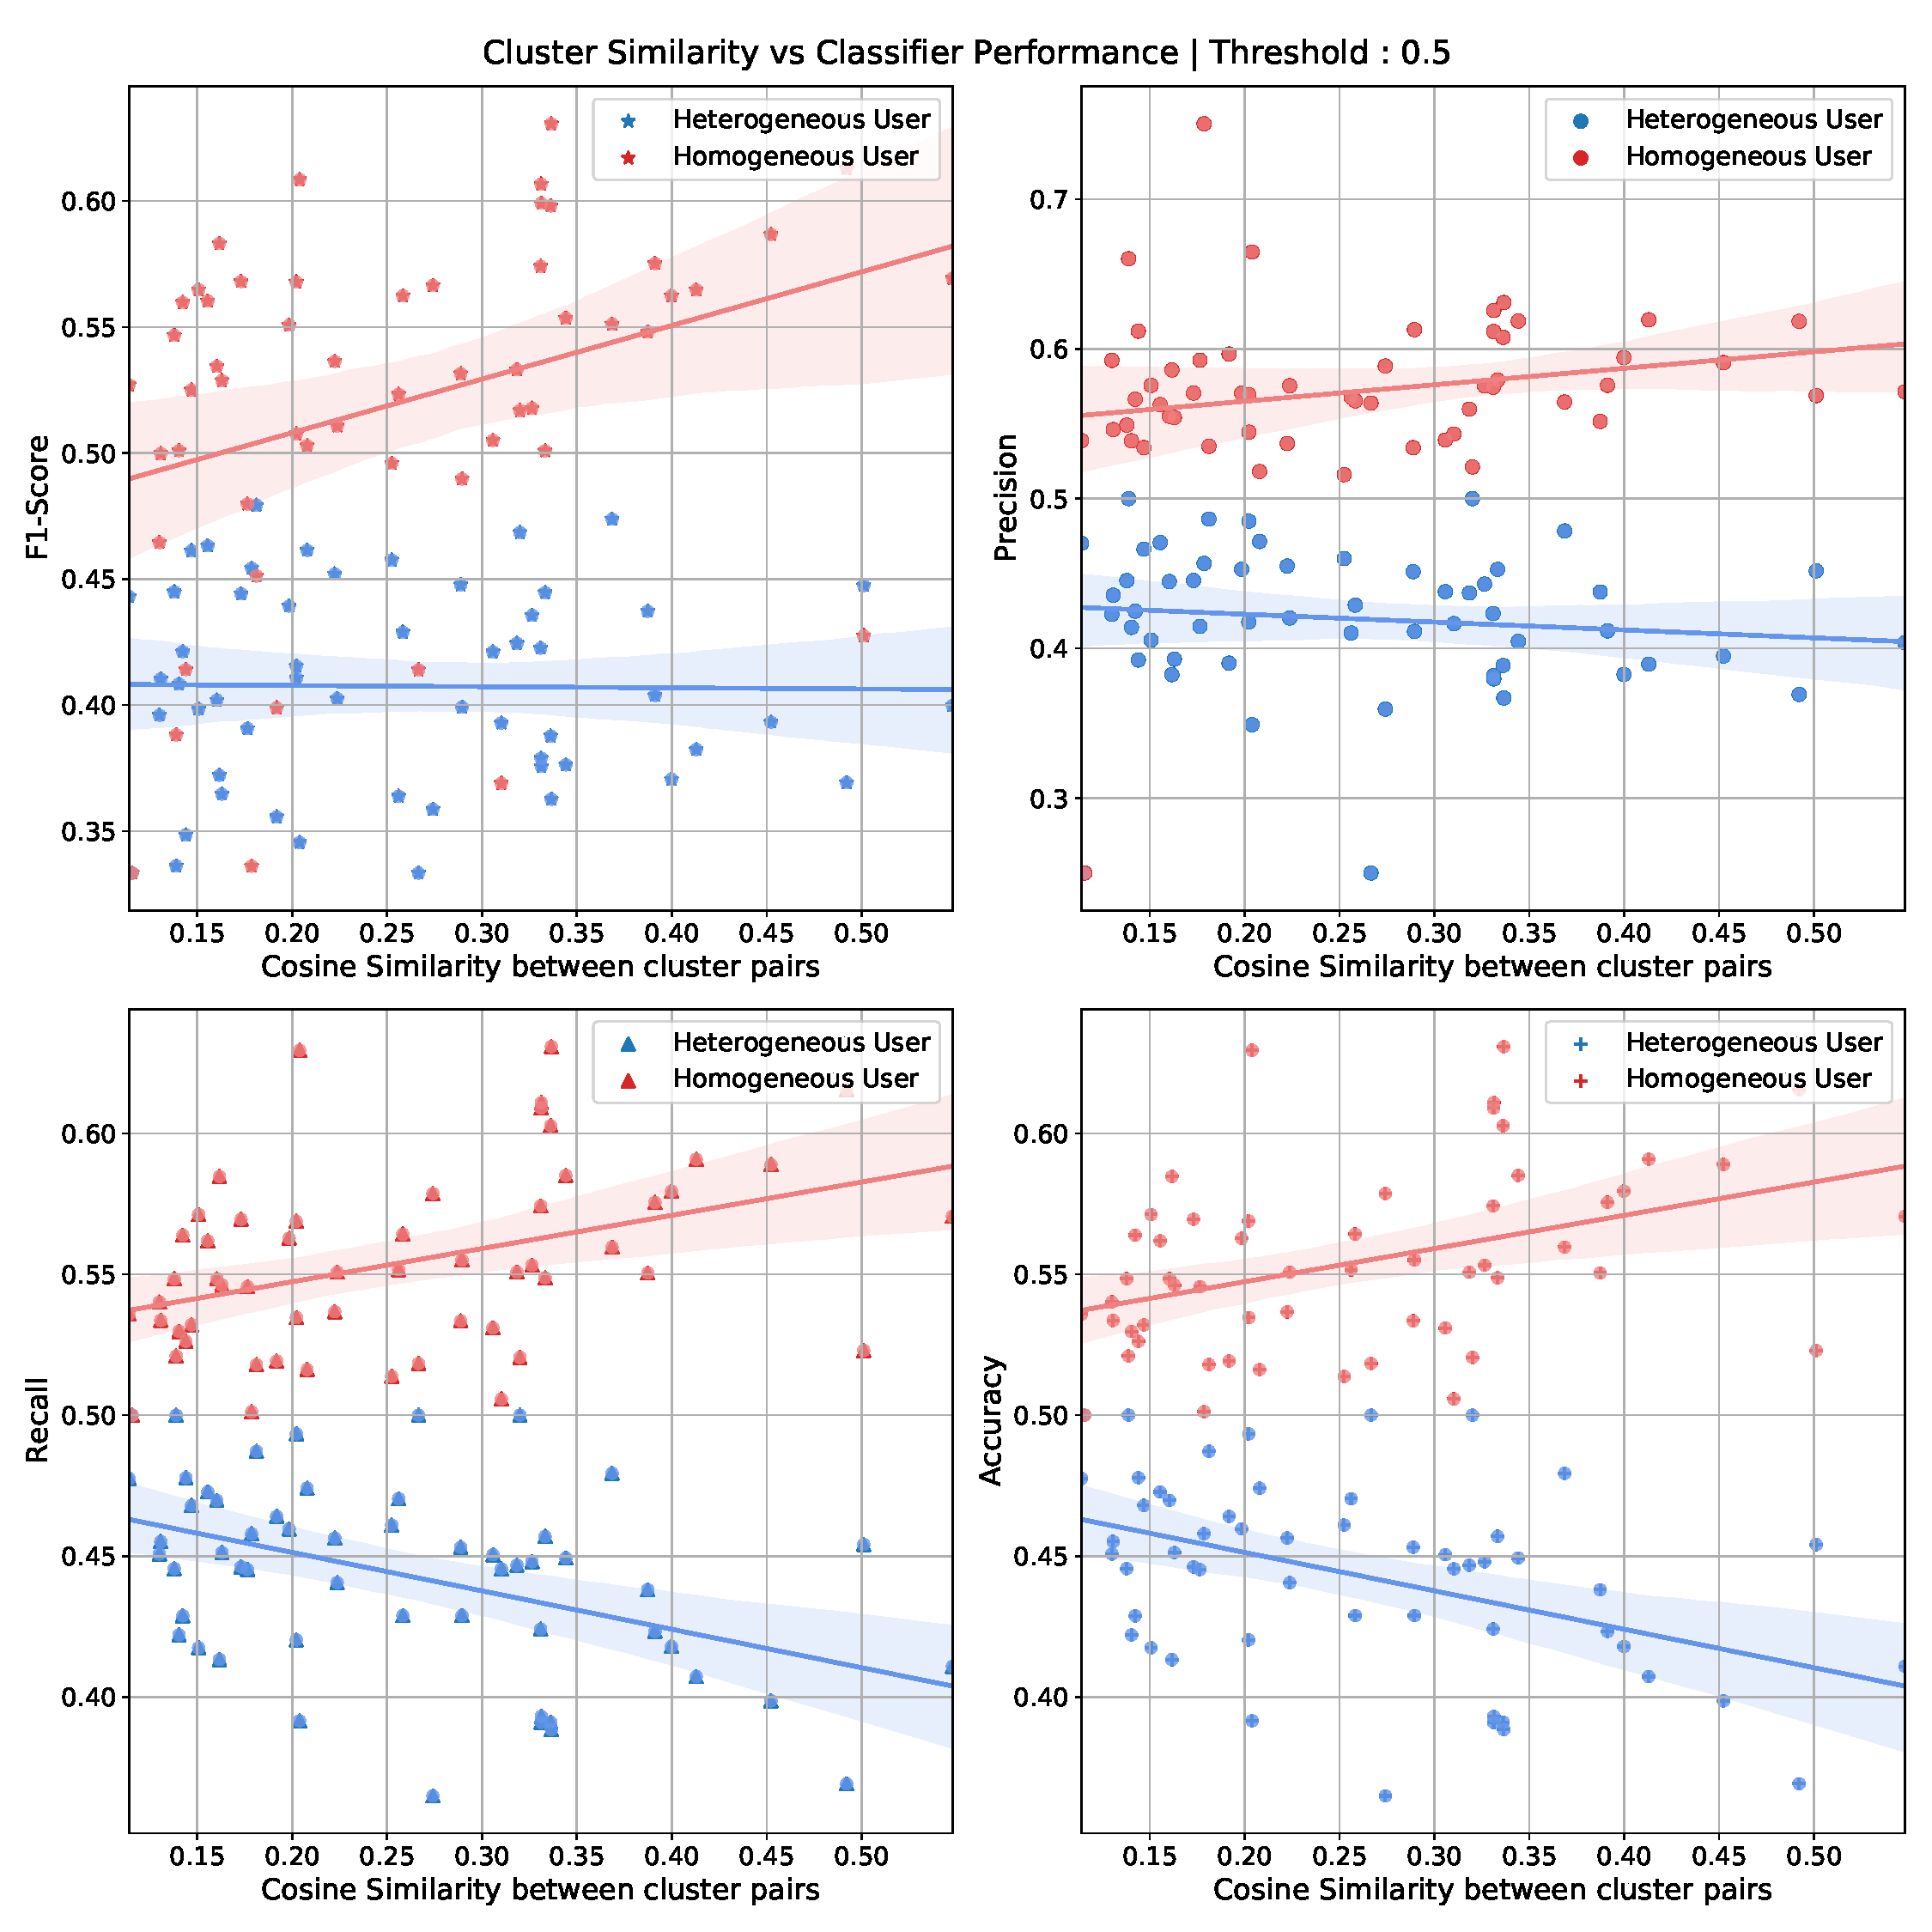
\includegraphics[width=0.8\textwidth]{Graphs/cluster_sim_vs_model_perf_5.pdf}
\end{figure}
\subsection{Observations :}
\begin{flushleft}
\textbf{Note :} The metrics measured for this baseline experiment is based on a test set and not calculated at a particular time step or user-interaction
\begin{itemize}
    \item We see that for homogeneous user's there is an increase in \textbf{Precision} and \textbf{Recall} when similarity between the clusters/topics increases.
    \item For a Heterogeneous User we see the opposite effect with a slight decrease in \textbf{Precision} and a larger decrease in \textbf{Recall} as cosine similarity between the topics or clusters increase suggesting the difficulty in distinguishing between really similar articles of conservative and liberal stance for the content recommendation system.
\end{itemize}
\end{flushleft}



\vspace{-1ex}
\section{Baseline 2: Online Learning Setting}
\begin{flushleft}
To emulate a real-world scenario , we want to simulate a recommendation system interacting with a user over a set of unseen articles , slowly updating itself to learn the user's preferences over time, \textbf{N=200} is used here to calculate the metrics, where \textbf{N }represents the number of interactions between the user and the content recommender. Also to note, there are at least N relevant articles in the candidate pool. 
\end{flushleft}
\subsection{Online Metrics :}
\begin{flushleft}
For this baseline experiment we use recommender specific metrics such as \textbf{Precision@K} and \textbf{Recall@K}.
\begin{itemize}
    \item $Precision@K = \frac{\# recommended \; items \: the \: user \; likes \: at \: K_{th} \: Interaction}{total \: \#  \: of \: items \:  recommended \: at \: K_{th} \: Interaction}$
    
    \item $Recall@K = \frac{\# recommended \; items \: the \: user \; likes \: at \: K_{th} \; Interaction}{total \; \# of \; relevant \; items \; in \; the \; candidate \; pool}$
    
    \item Eg:  \begin{itemize}
        \item Candidate Pool Size = 15
        \item Number of relevant(user-likes) items in the candidate pool = 10
        \item N = 1 \begin{itemize}
            \item Shown Articles = [0]
            \item Recall = 0/10 = 0
            \item Precision = 0/1 = 0
        \end{itemize}
        \item N = 2 \begin{itemize}
            \item Shown Articles = [0,1]
            \item Recall = 1/10 = 0.1
            \item Precision = 1/2 = 0.5
        \end{itemize}
        \item N = 3 \begin{itemize}
            \item Shown Articles = [0,1,1]
            \item Recall = 2/10 = 0.2
            \item Precision = 2/3 = 0.666
        \end{itemize}
        \item N = 4 \begin{itemize}
            \item Shown Articles = [0,1,1,1]
            \item Recall = 3/10 = 0.3
            \item Precision = 3/4 = 0.75
        \end{itemize}
    \end{itemize}
    
\end{itemize}
\end{flushleft}

\vspace{1ex}
\begin{figure}[H]
 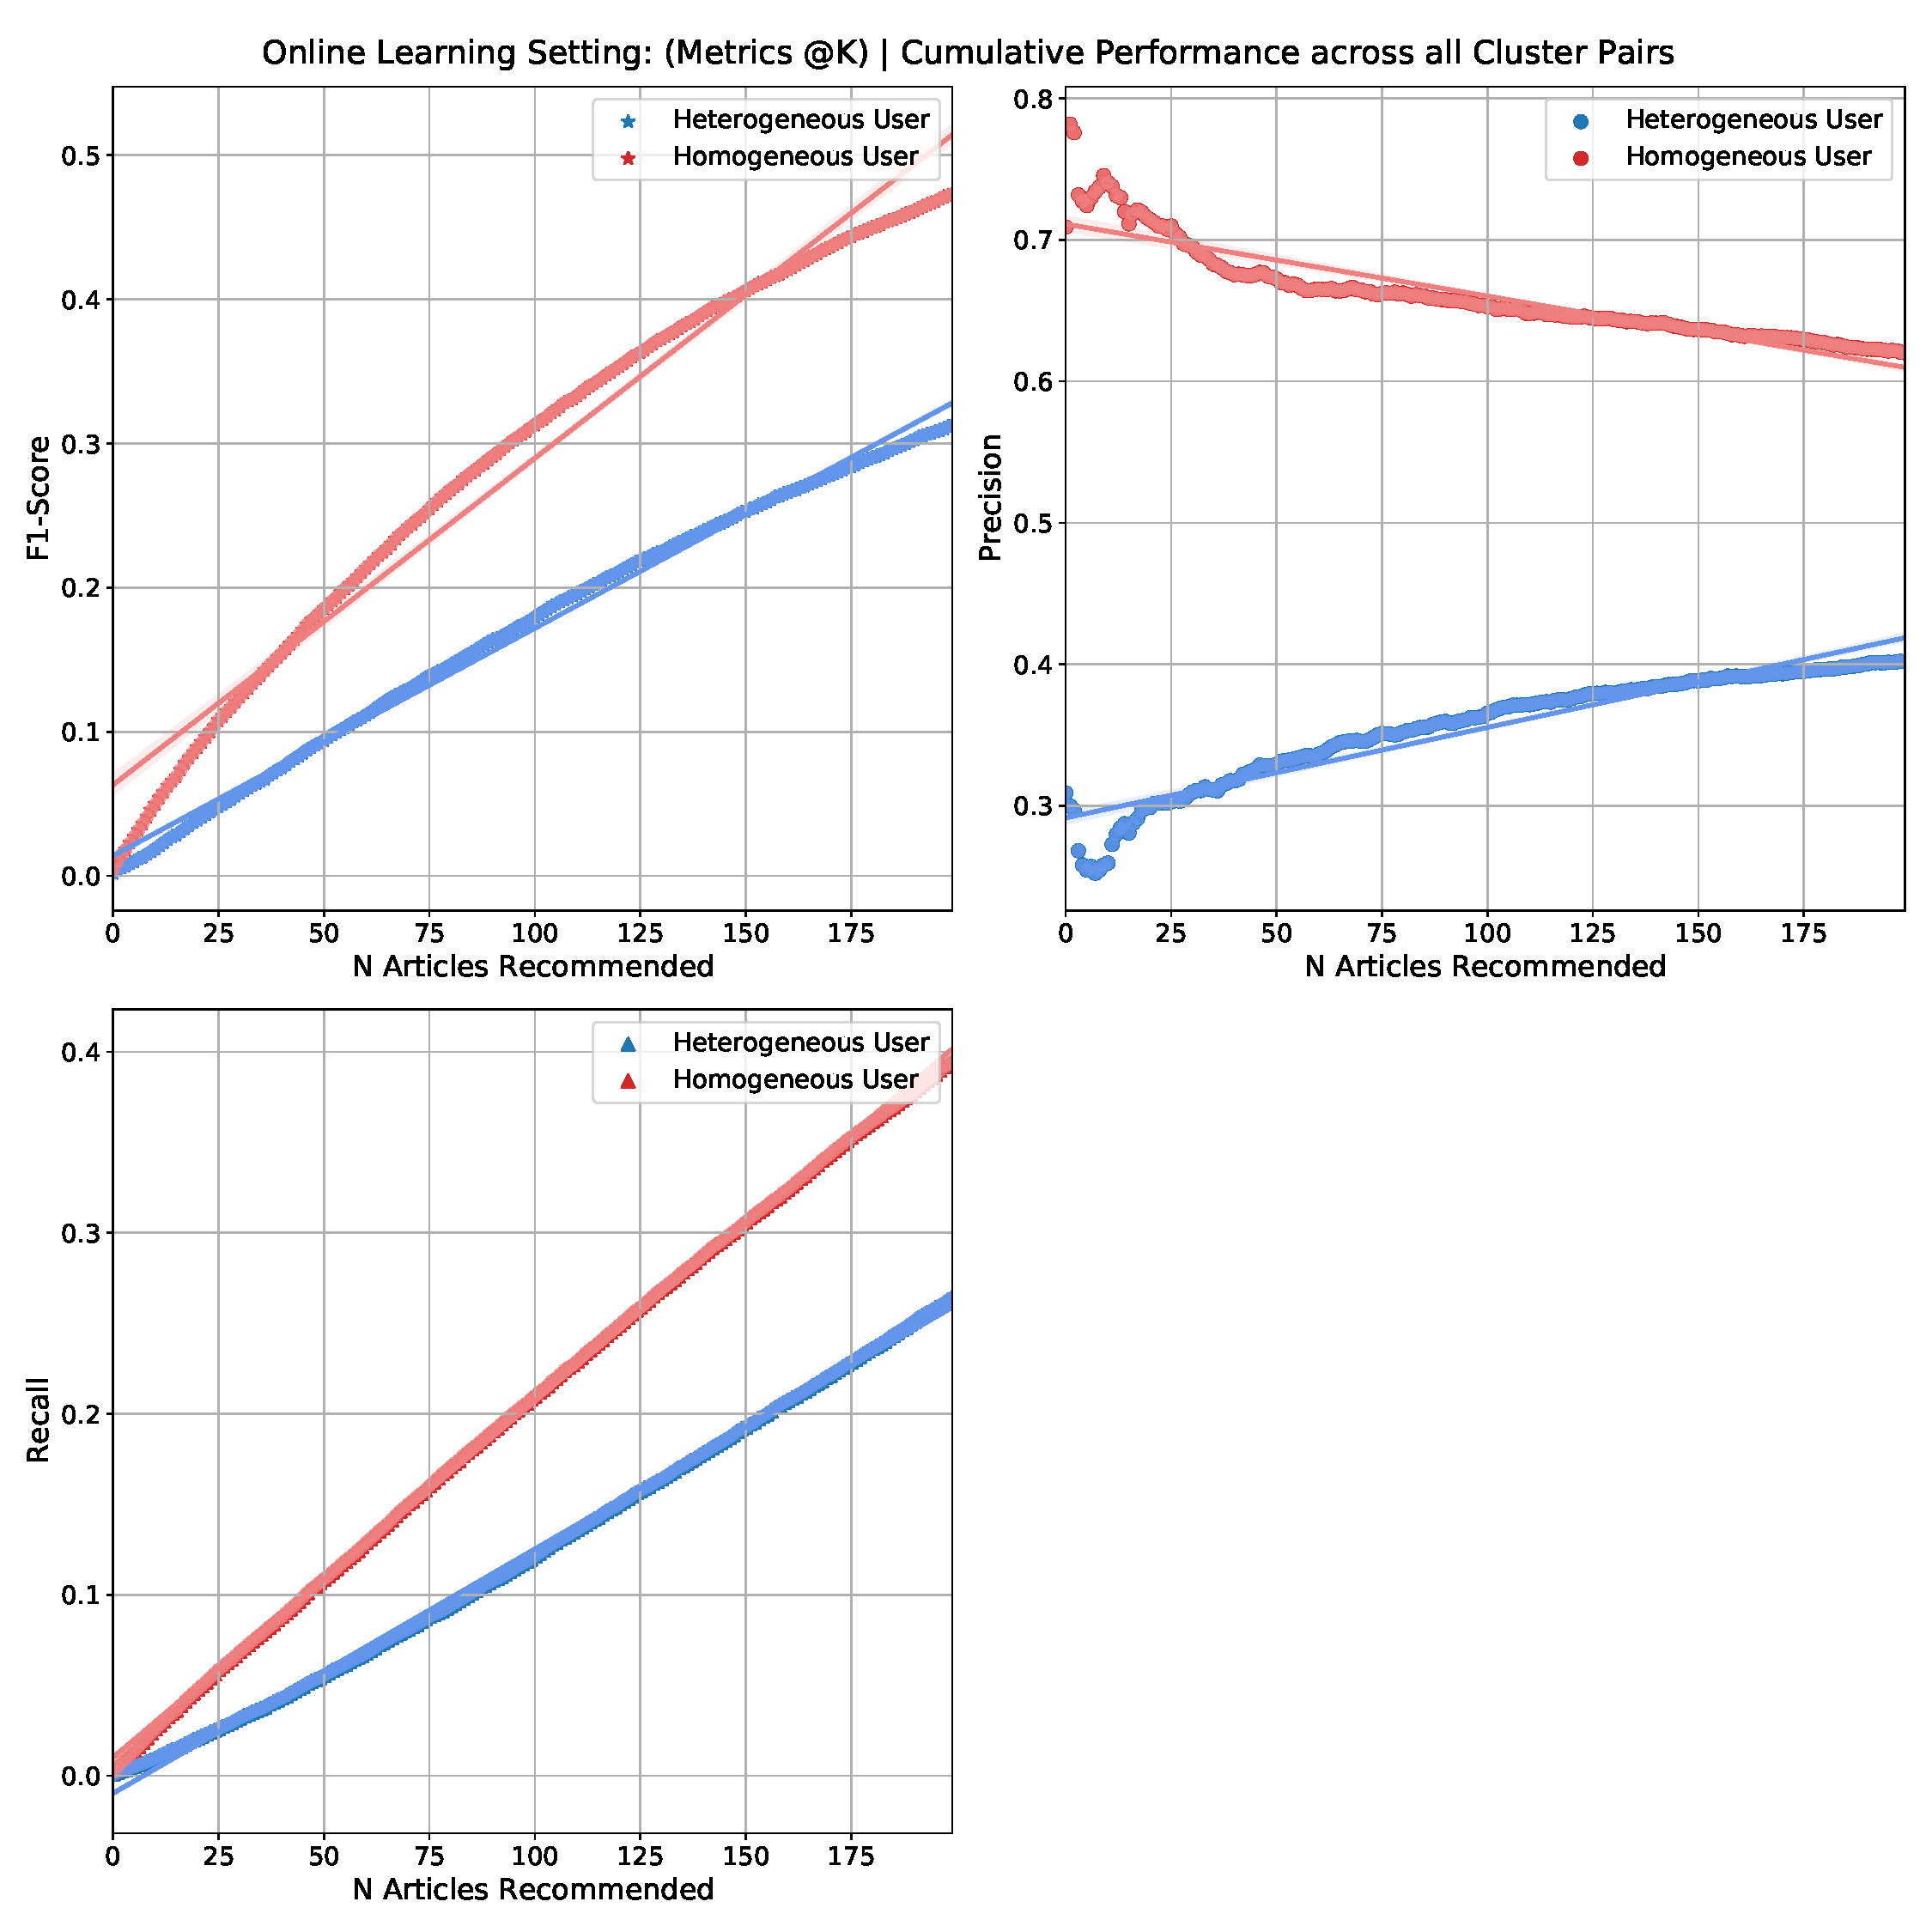
\includegraphics[width=0.8\textwidth]{Graphs/user_interaction_vs_model_performance_cumu.pdf}
\end{figure}
\vspace{-4ex}
\begin{figure}[H]
 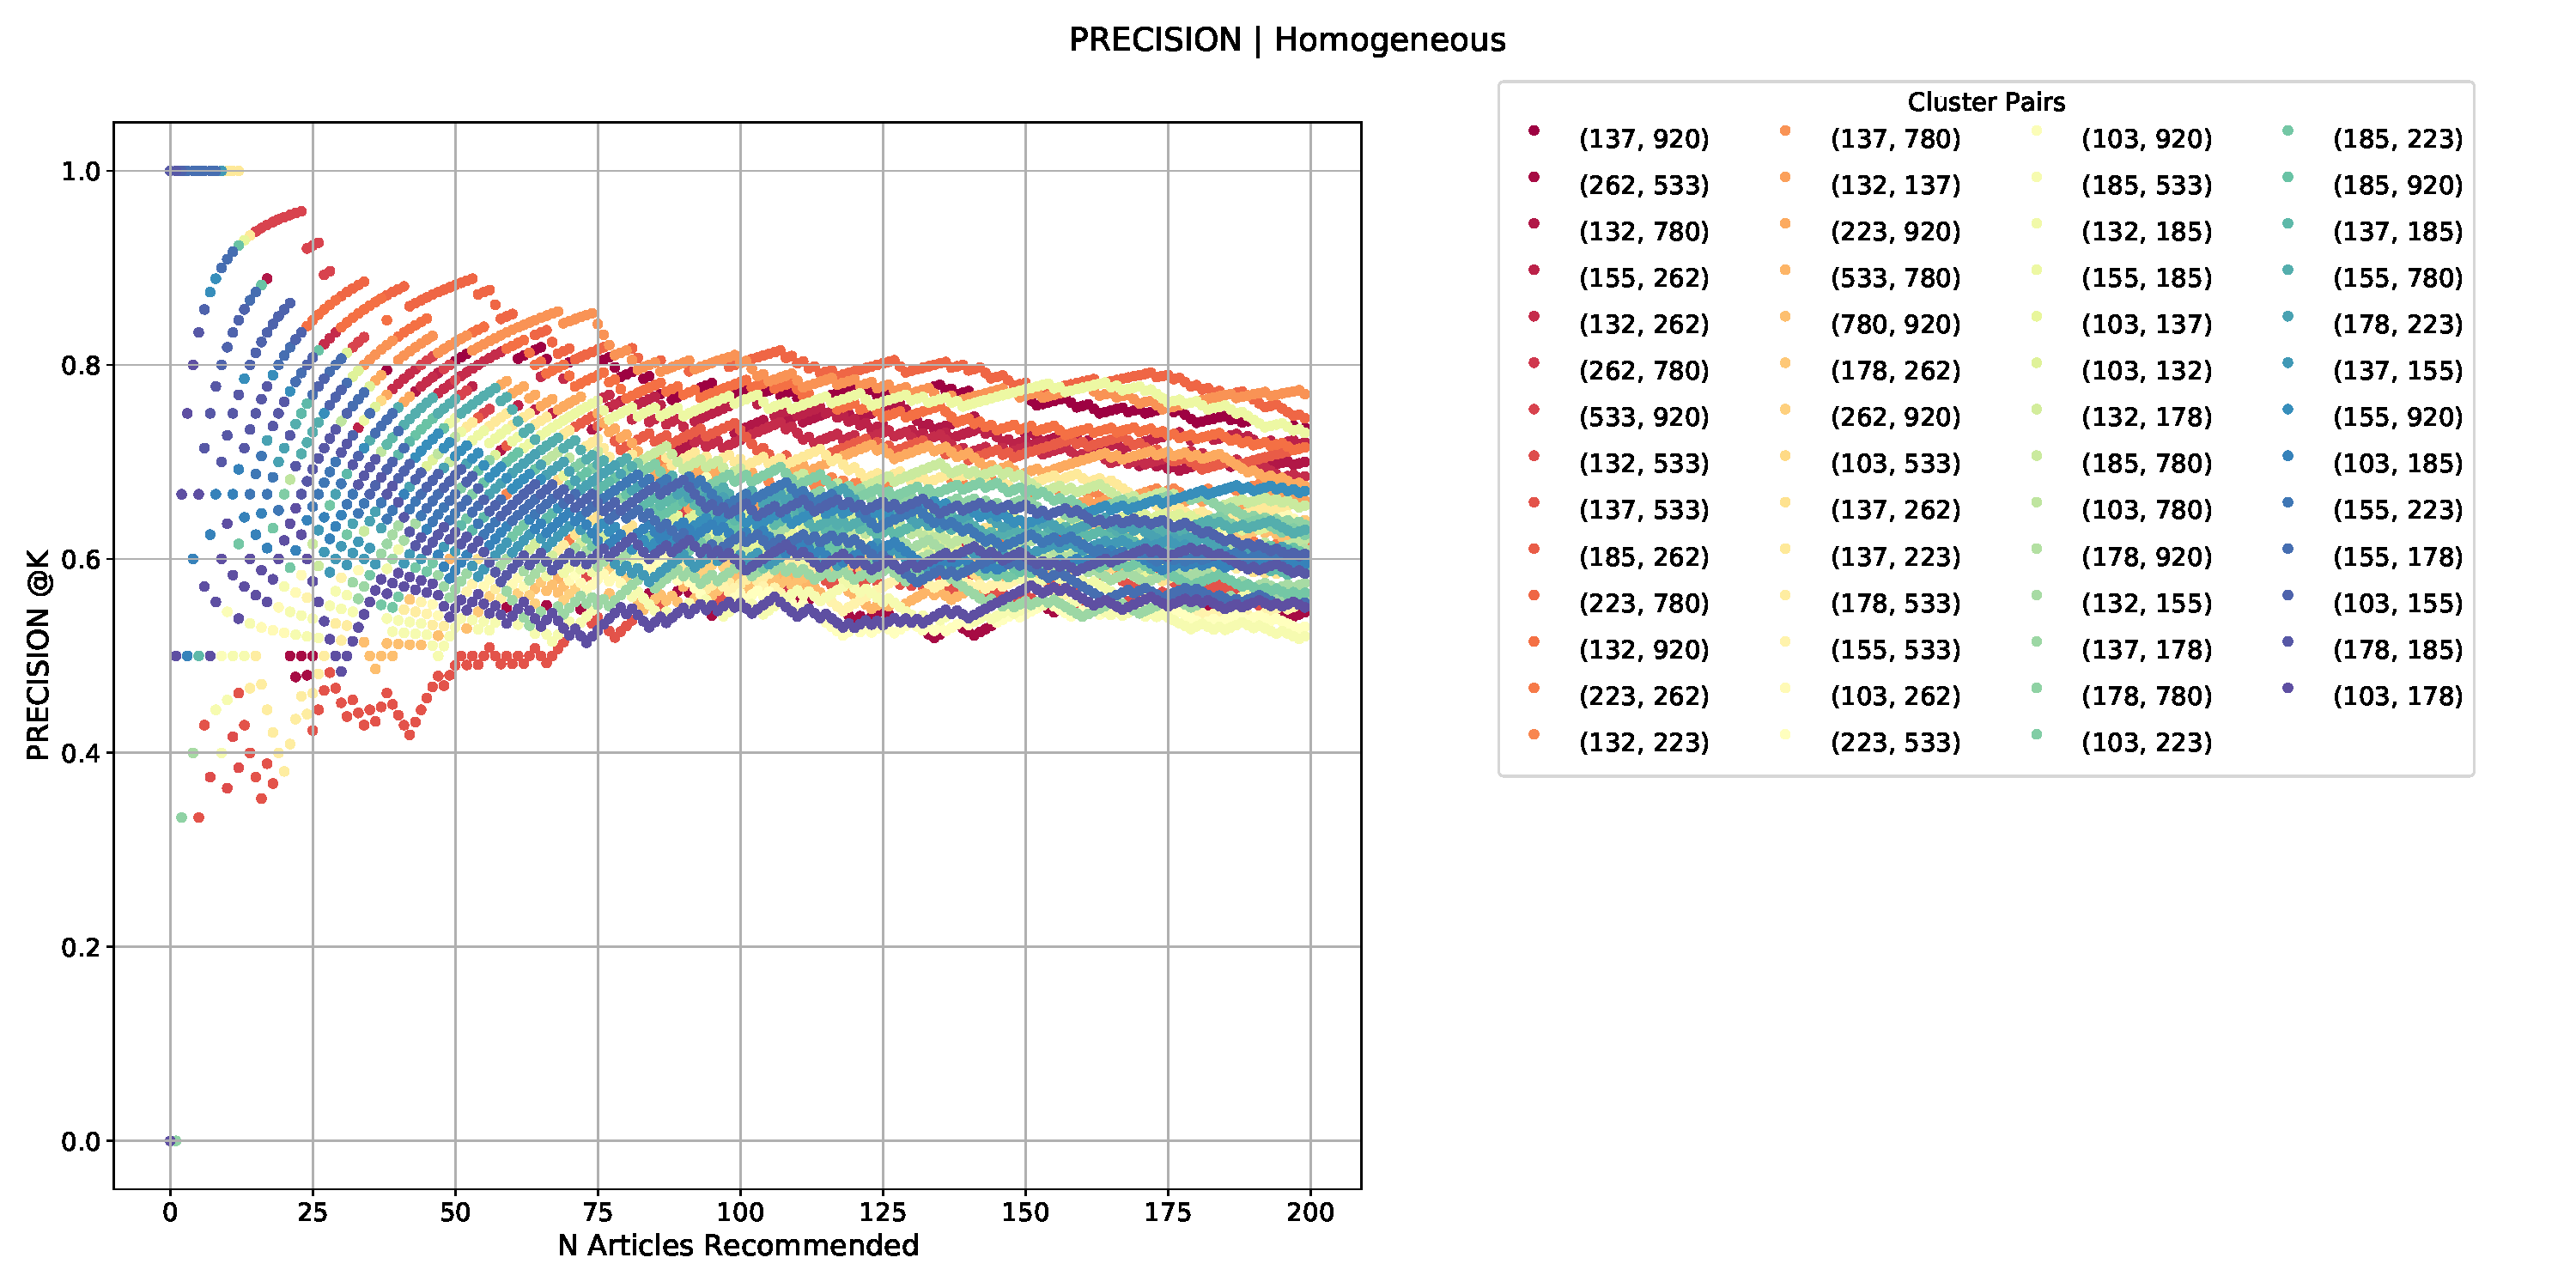
\includegraphics[width=1.0\textwidth]{Graphs/user_interaction_vs_model_performance_precision_all_cps_Homogeneous.pdf}
\end{figure}
\begin{figure}[H]
 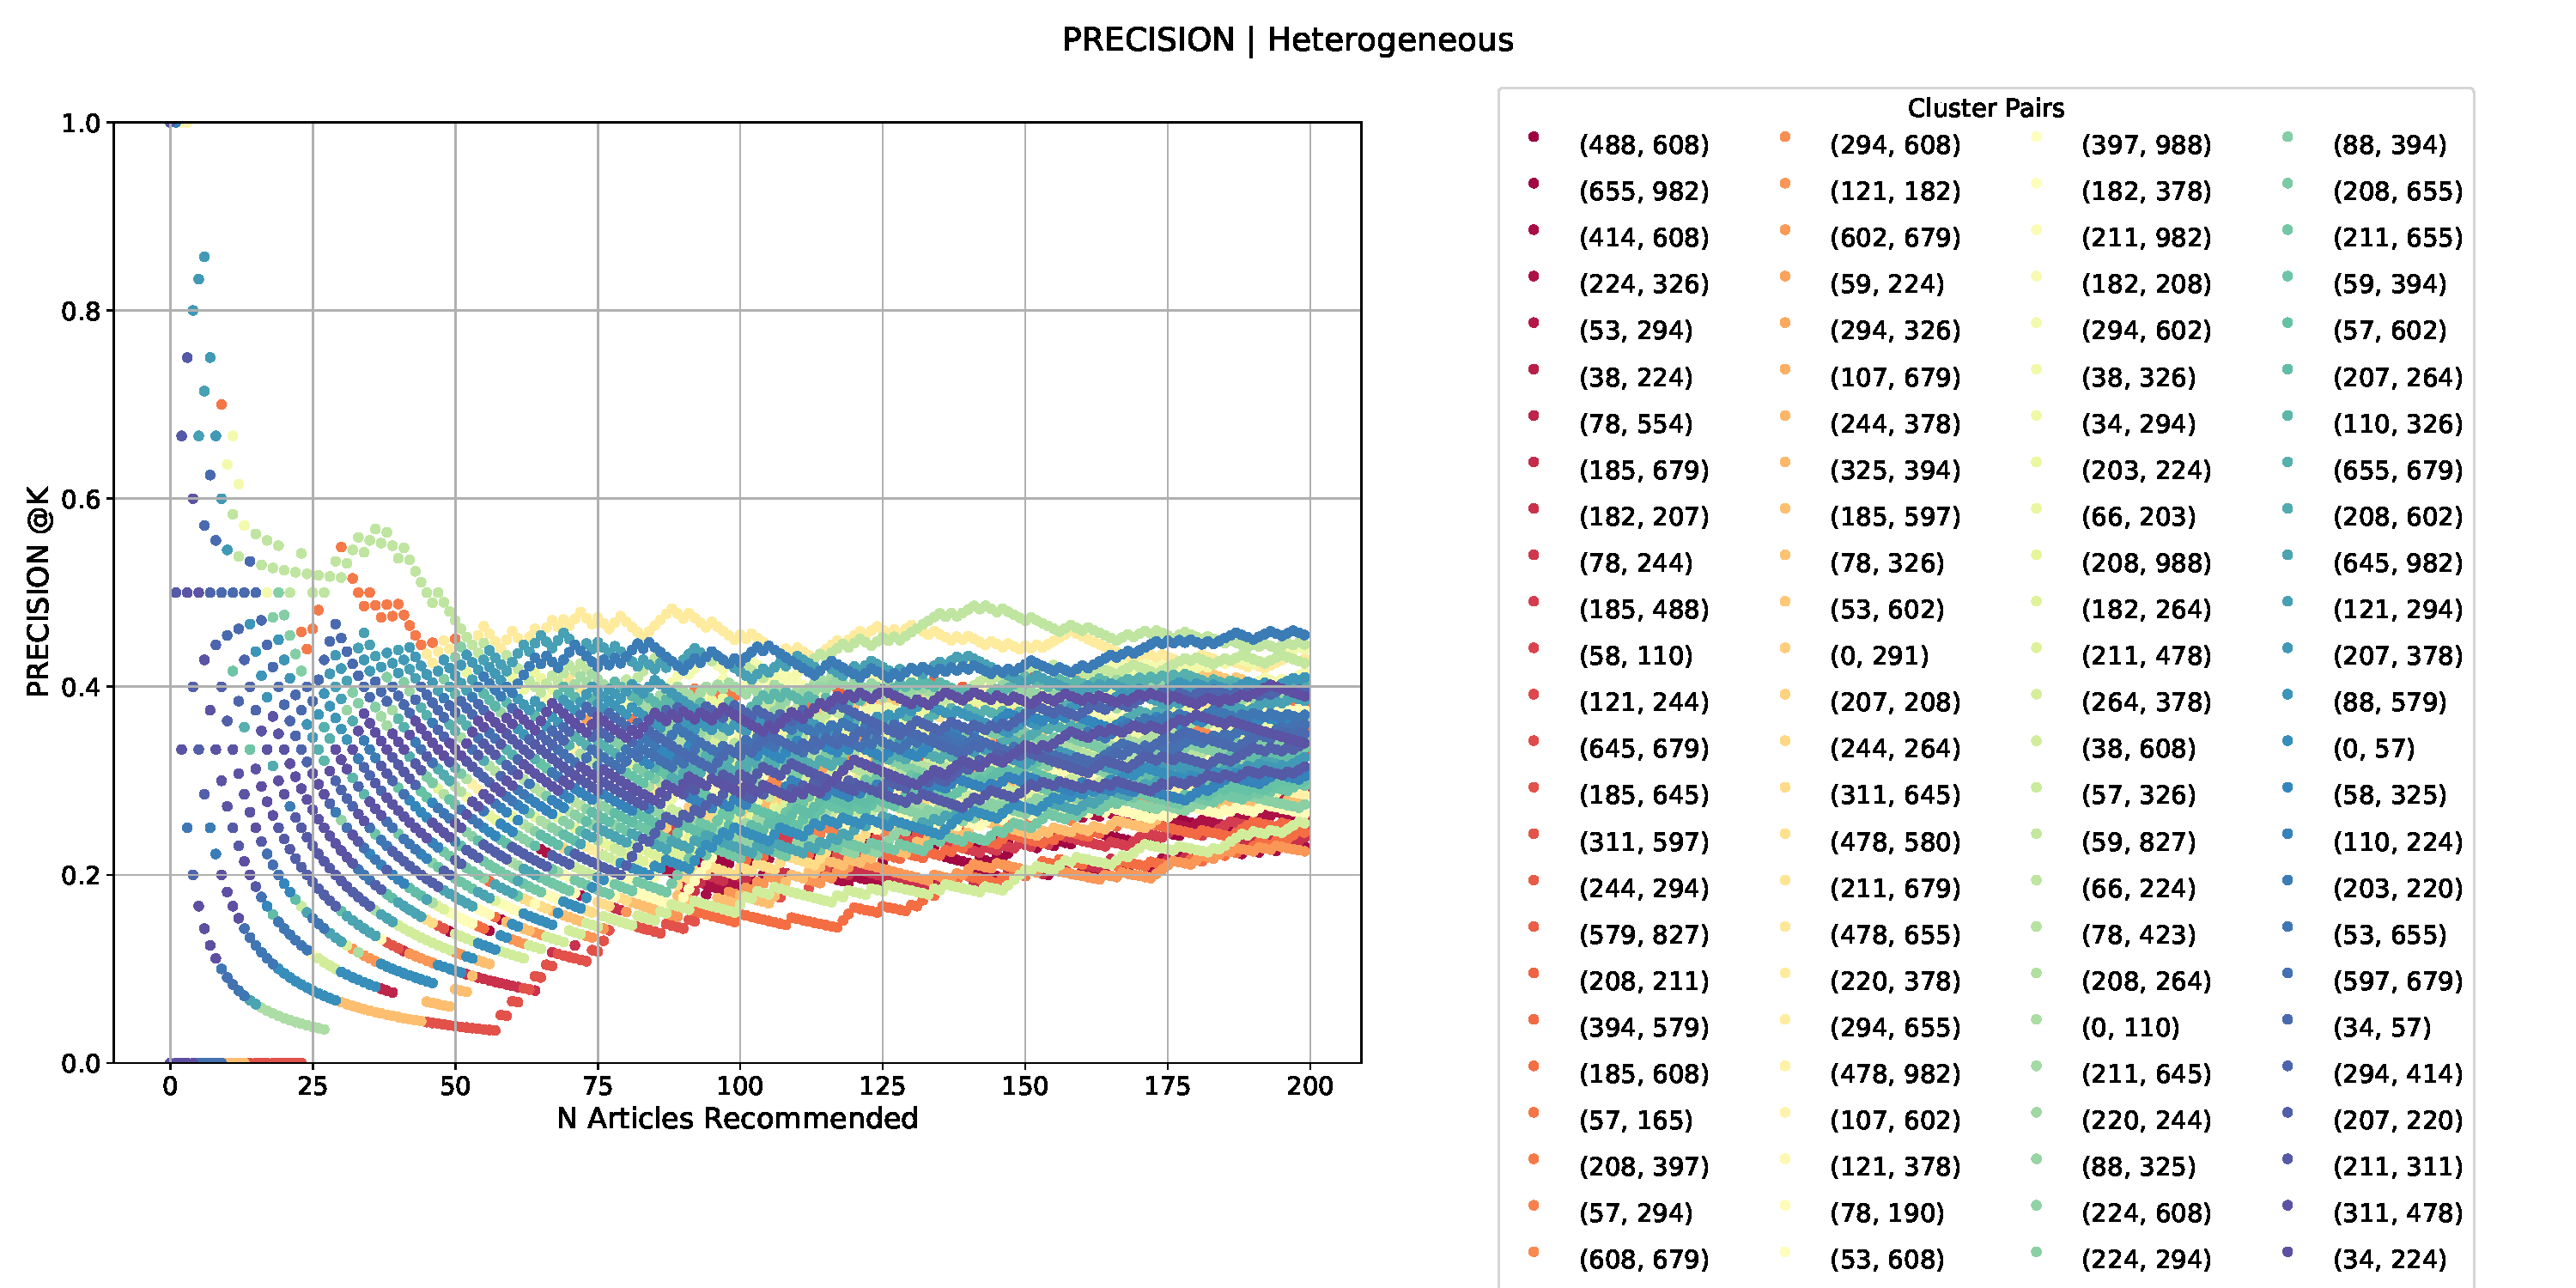
\includegraphics[width=1.0\textwidth]{Graphs/user_interaction_vs_model_performance_precision_all_cps_Heterogeneous.pdf}
\end{figure}
\subsection{Observations:}
\begin{flushleft}
The above figure shows the mean results across all cluster pairs.
\begin{itemize}
    \item For the Homogeneous User we see that \textbf{Precision@K} decreases as the number of interactions increase, this could be due to the fact that the most probable items the user likes are already recommended in the initial user-interactions (as we sort by predicted probability). Also from the precision graph with all cluster pairs shown we see that a few clusters do increase in precision.
    \item For the Heterogeneous User we see that their is an initial dip in \textbf{Precision@K} and then it increases as the content recommender learns the different preferences of the heterogeneous user.
    \item We also see that the \textbf{Recall@K} increases as number of interactions increase (as more relevant articles keep getting recommended).
    \item Overall we see that the precision for Homogeneous users is higher than heterogeneous users
\end{itemize}
\end{flushleft}


\vspace{-1ex}
\newpage
\section{Baseline 3: How easy is it for the Recommendation System to detect a change in topics}
\begin{flushleft}
We want to know how the recommendation system performs in detecting a change in topics , so we measure the performance of the system using a single cluster and compare it against our online setting performance (shown in the above baseline). 
\end{flushleft}
\subsection{Observations :}
\begin{flushleft}
\begin{itemize}
    \item Similar trend in Precision@K occurs here (compared to baseline 2 - Homogeneous User). 
    \item  When we compare these scores to graphs in Baseline 2 we definitely see that the recommendation system tends to have an easier time when only one topic is concerned compared to 2 different topics, so the model is having a hard time in identifying a change in topic.
\end{itemize}
\end{flushleft}
% \vspace{-5ex}
\begin{figure}[H]
 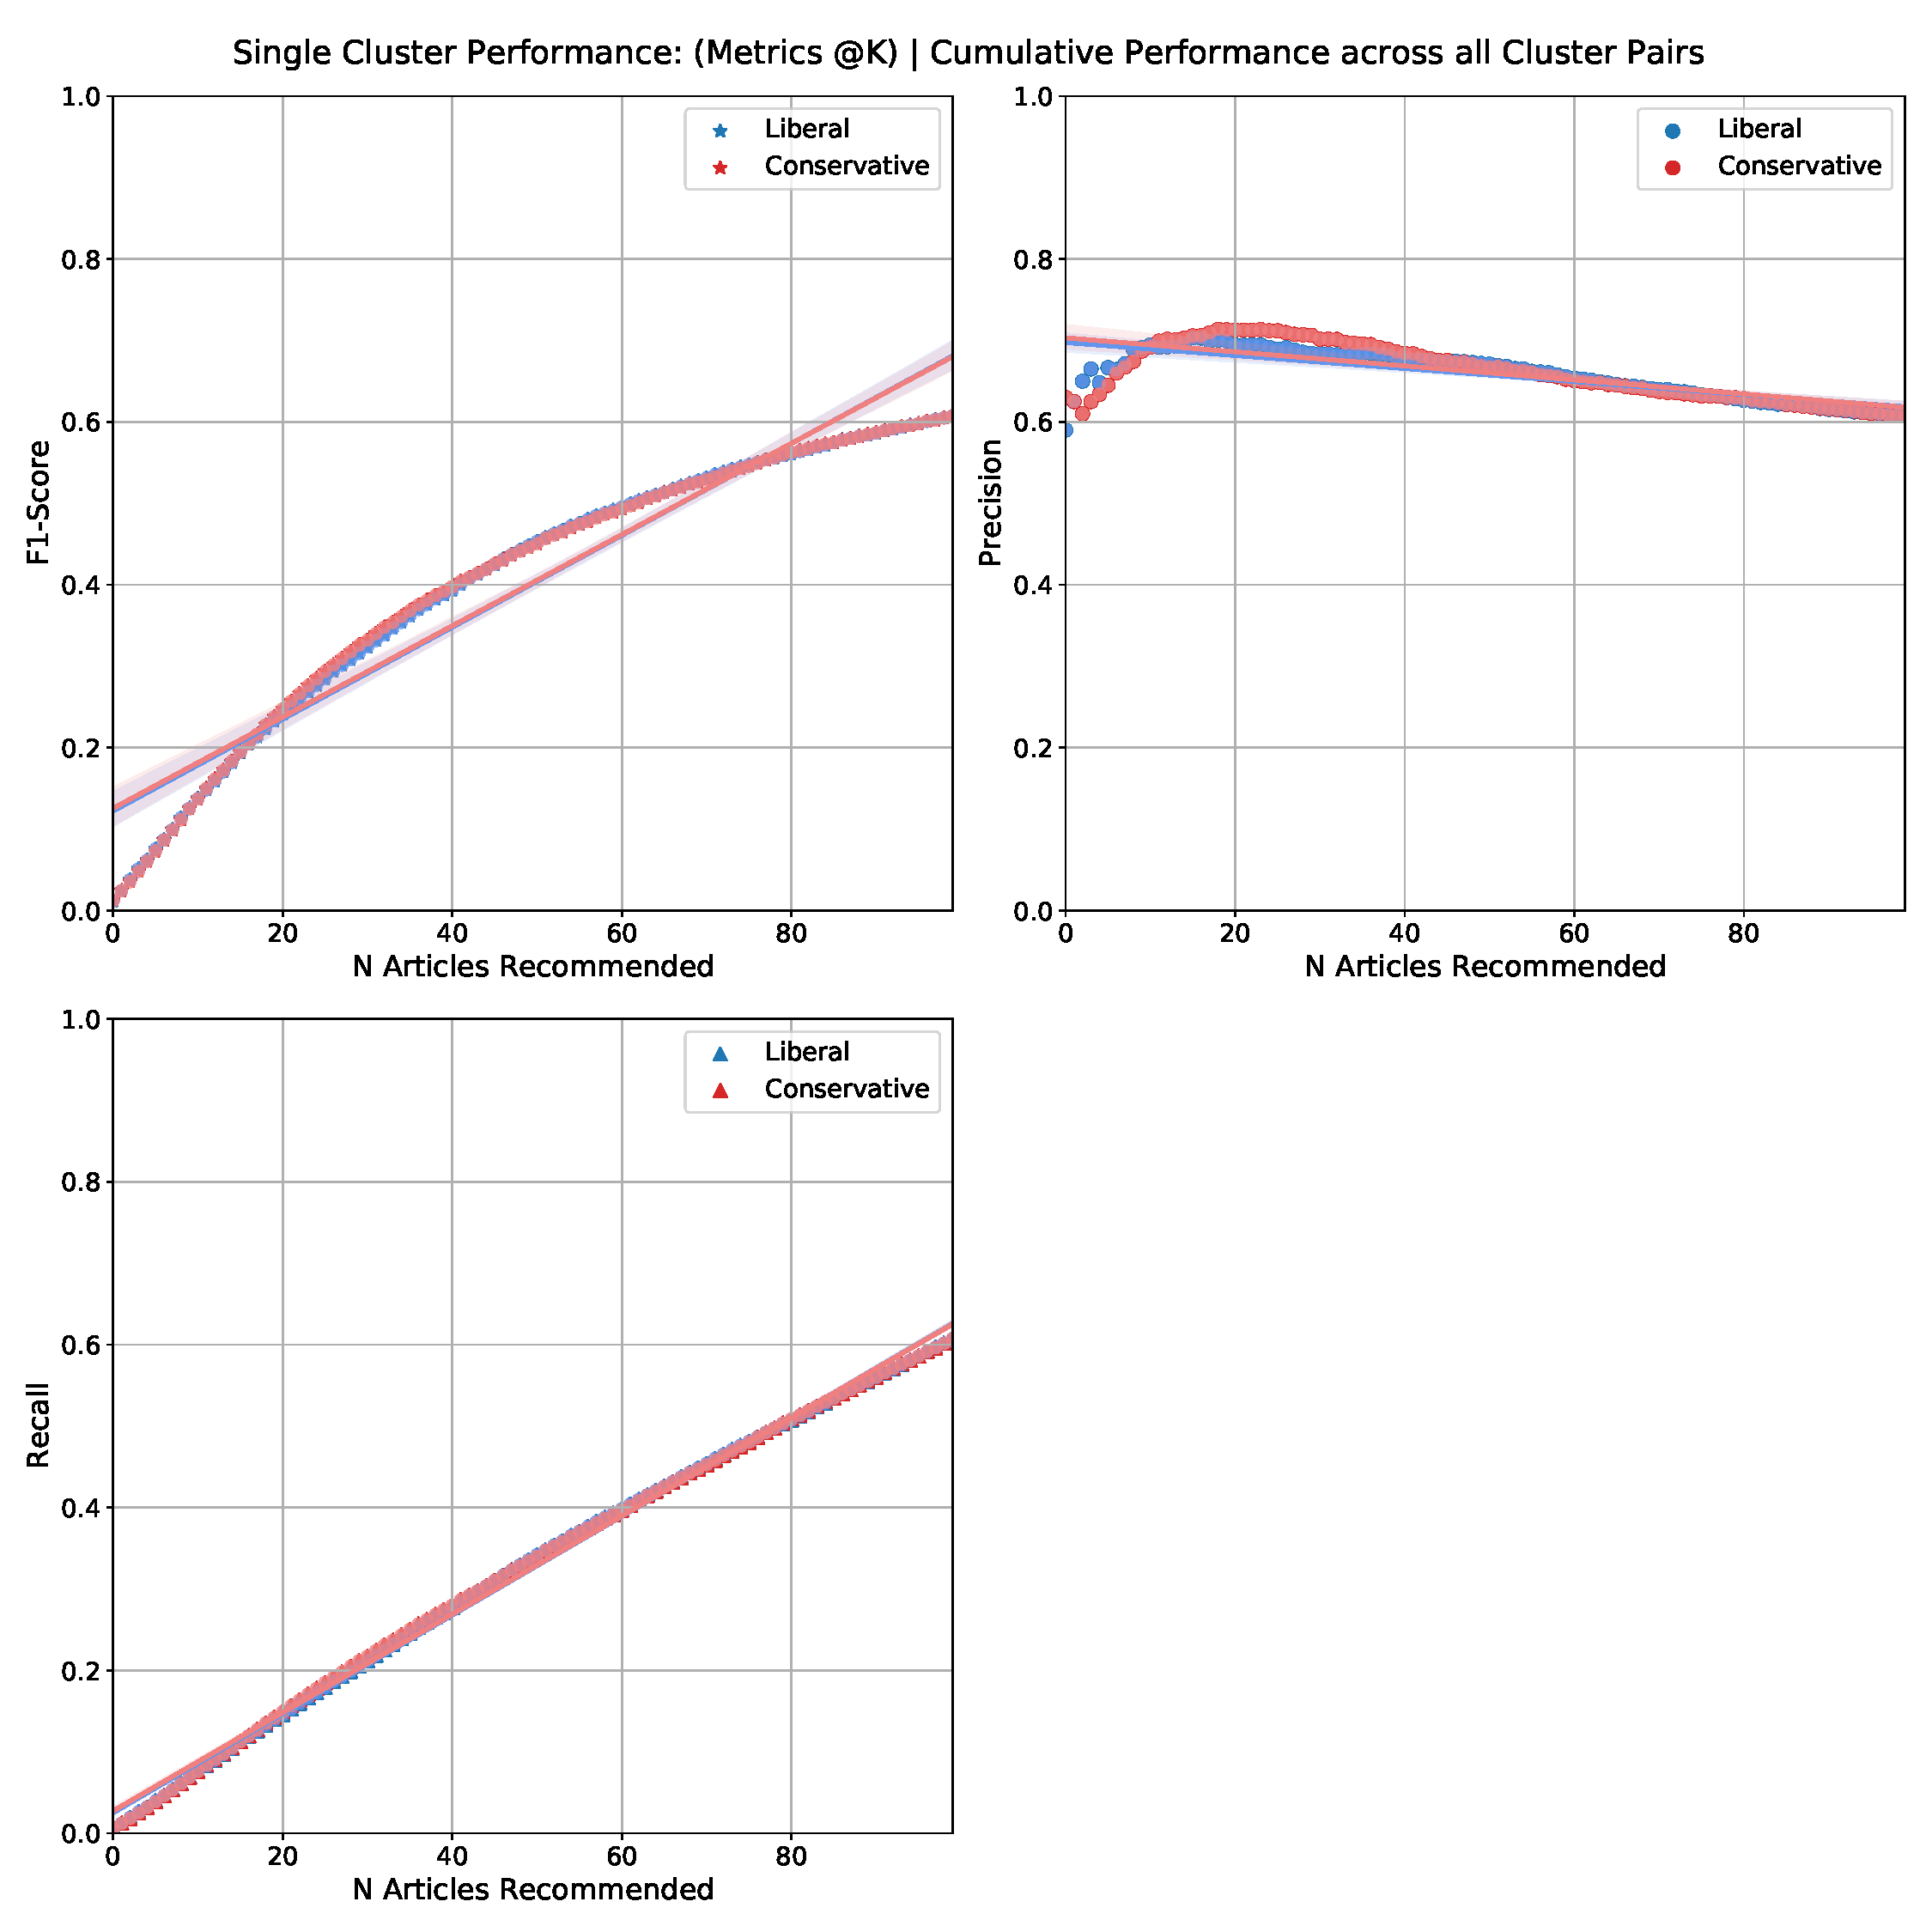
\includegraphics[width=0.8\textwidth]{Graphs/user_interaction_vs_model_performance_cumu_single_cluster.pdf}
\end{figure}
\begin{figure}[H]
 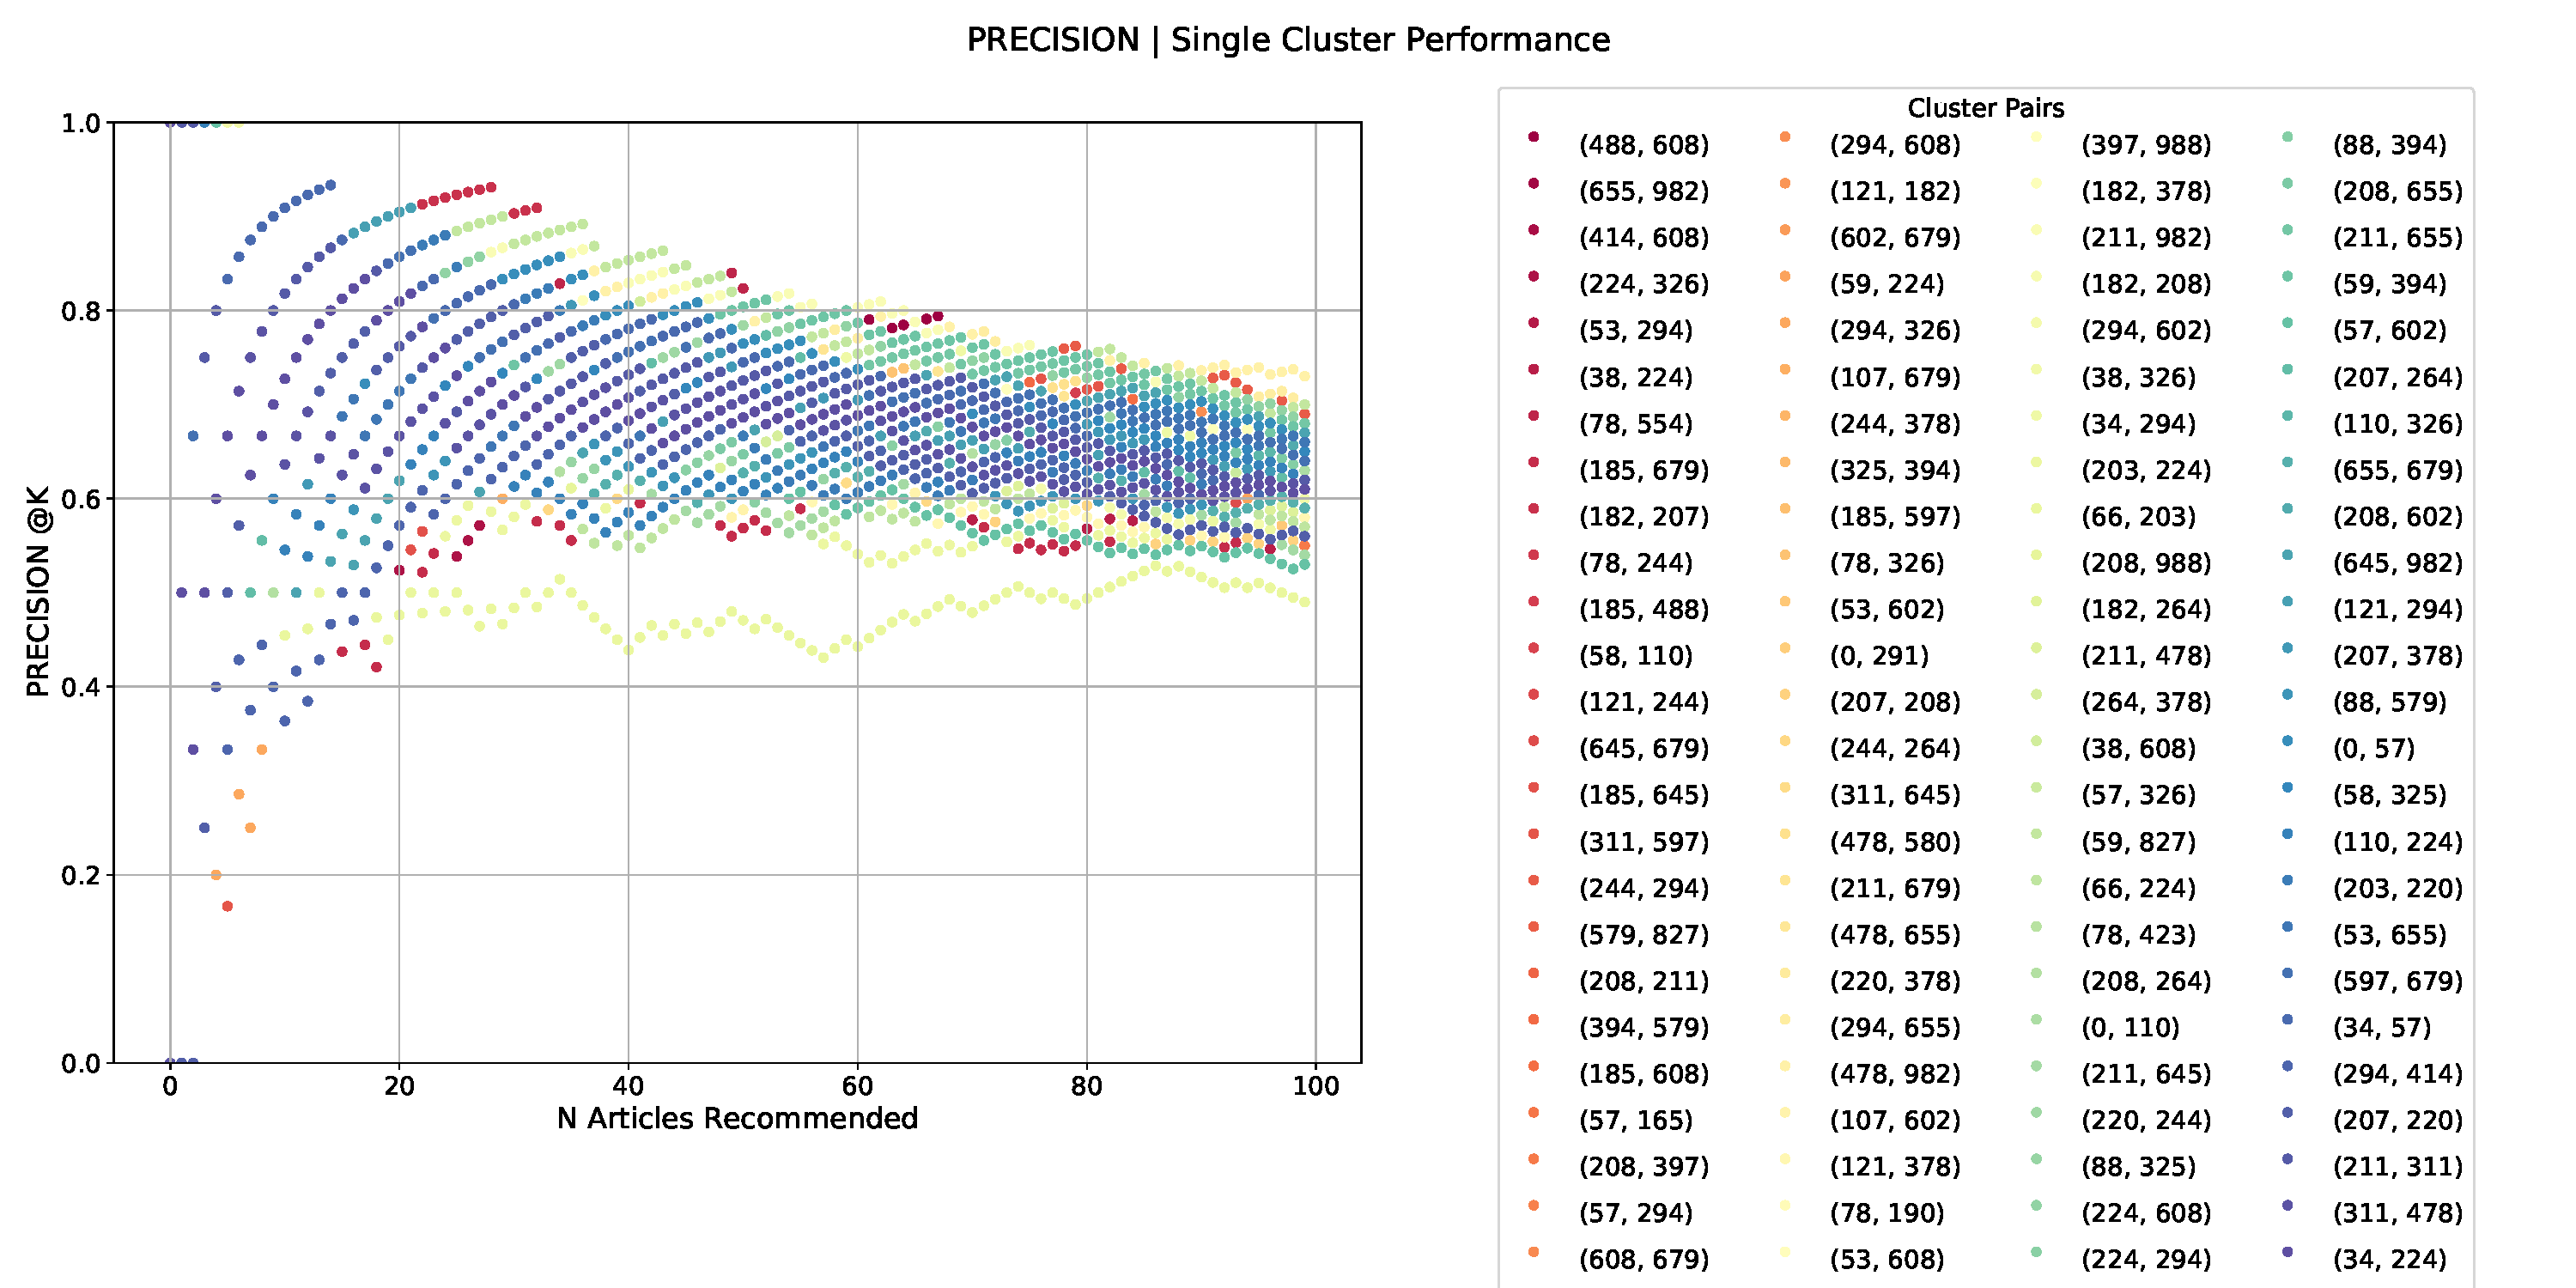
\includegraphics[width=1.0\textwidth]{Graphs/user_interaction_vs_model_performance_precision_all_cps_single_cluster.pdf}
\end{figure}




\section{Baseline 4: Varying Regularization Strength to remove Spurious Correlations}
\begin{flushleft}
We want to measure the effect of the size of regularization constant against model performance to see if removing spurious correlations helps aid model performance.

\subsection{Homogeneous Users}
\begin{flushleft}
For Homogeneous Users we see that a high regularization constant tends to hurt model performance, even not using a regularization constant (alpha =0) hurts precision compared to using a small regularization constant.
\end{flushleft}
\end{flushleft}
\vspace{-5ex}
\begin{figure}[H]
 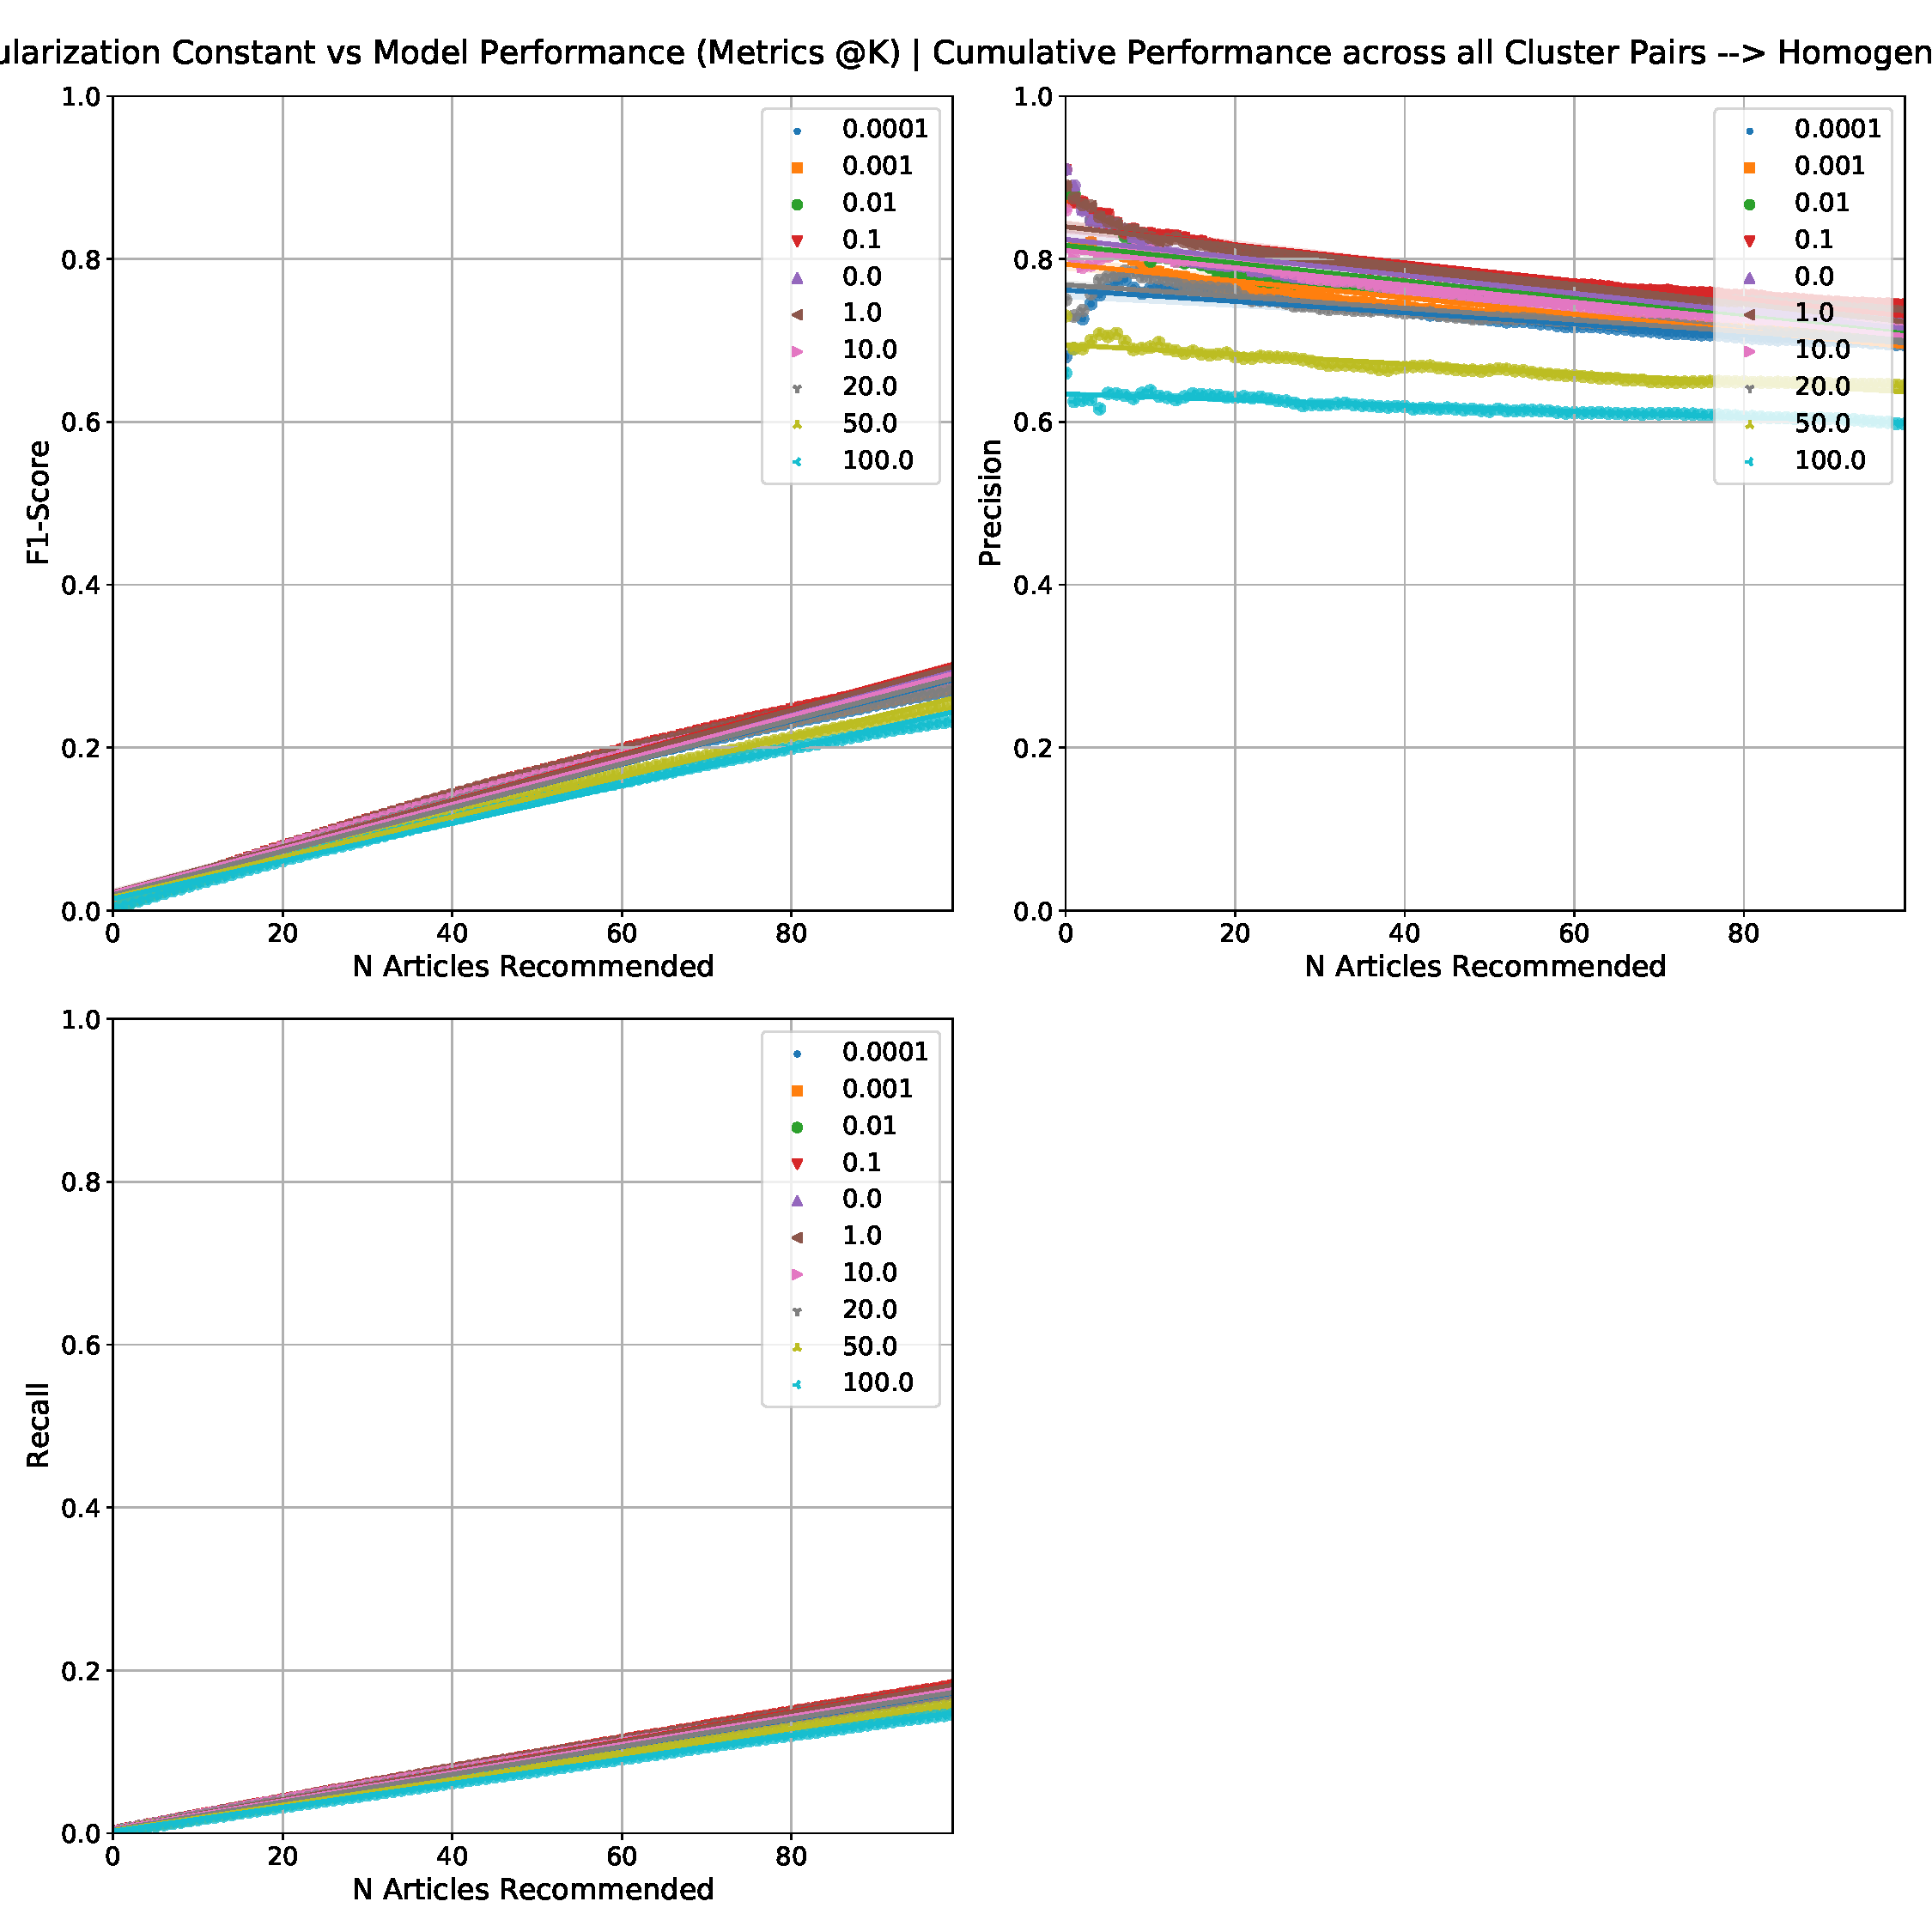
\includegraphics[width=0.8\textwidth]{Graphs/regularization_vs_model_performance_cumu_Homogeneous.pdf}
\end{figure}
\subsection{Heterogeneous Users}
\begin{flushleft}
For Heterogeneous Users on the other hand, the greater the regularization constant the better the model performs (as it can be seen across all 3 metrics), so limiting spurious correlations definitely does help in this scenario as words that overlap across stances are demoted in importance. 
\end{flushleft}
\vspace{-3ex}
\begin{figure}[H]
 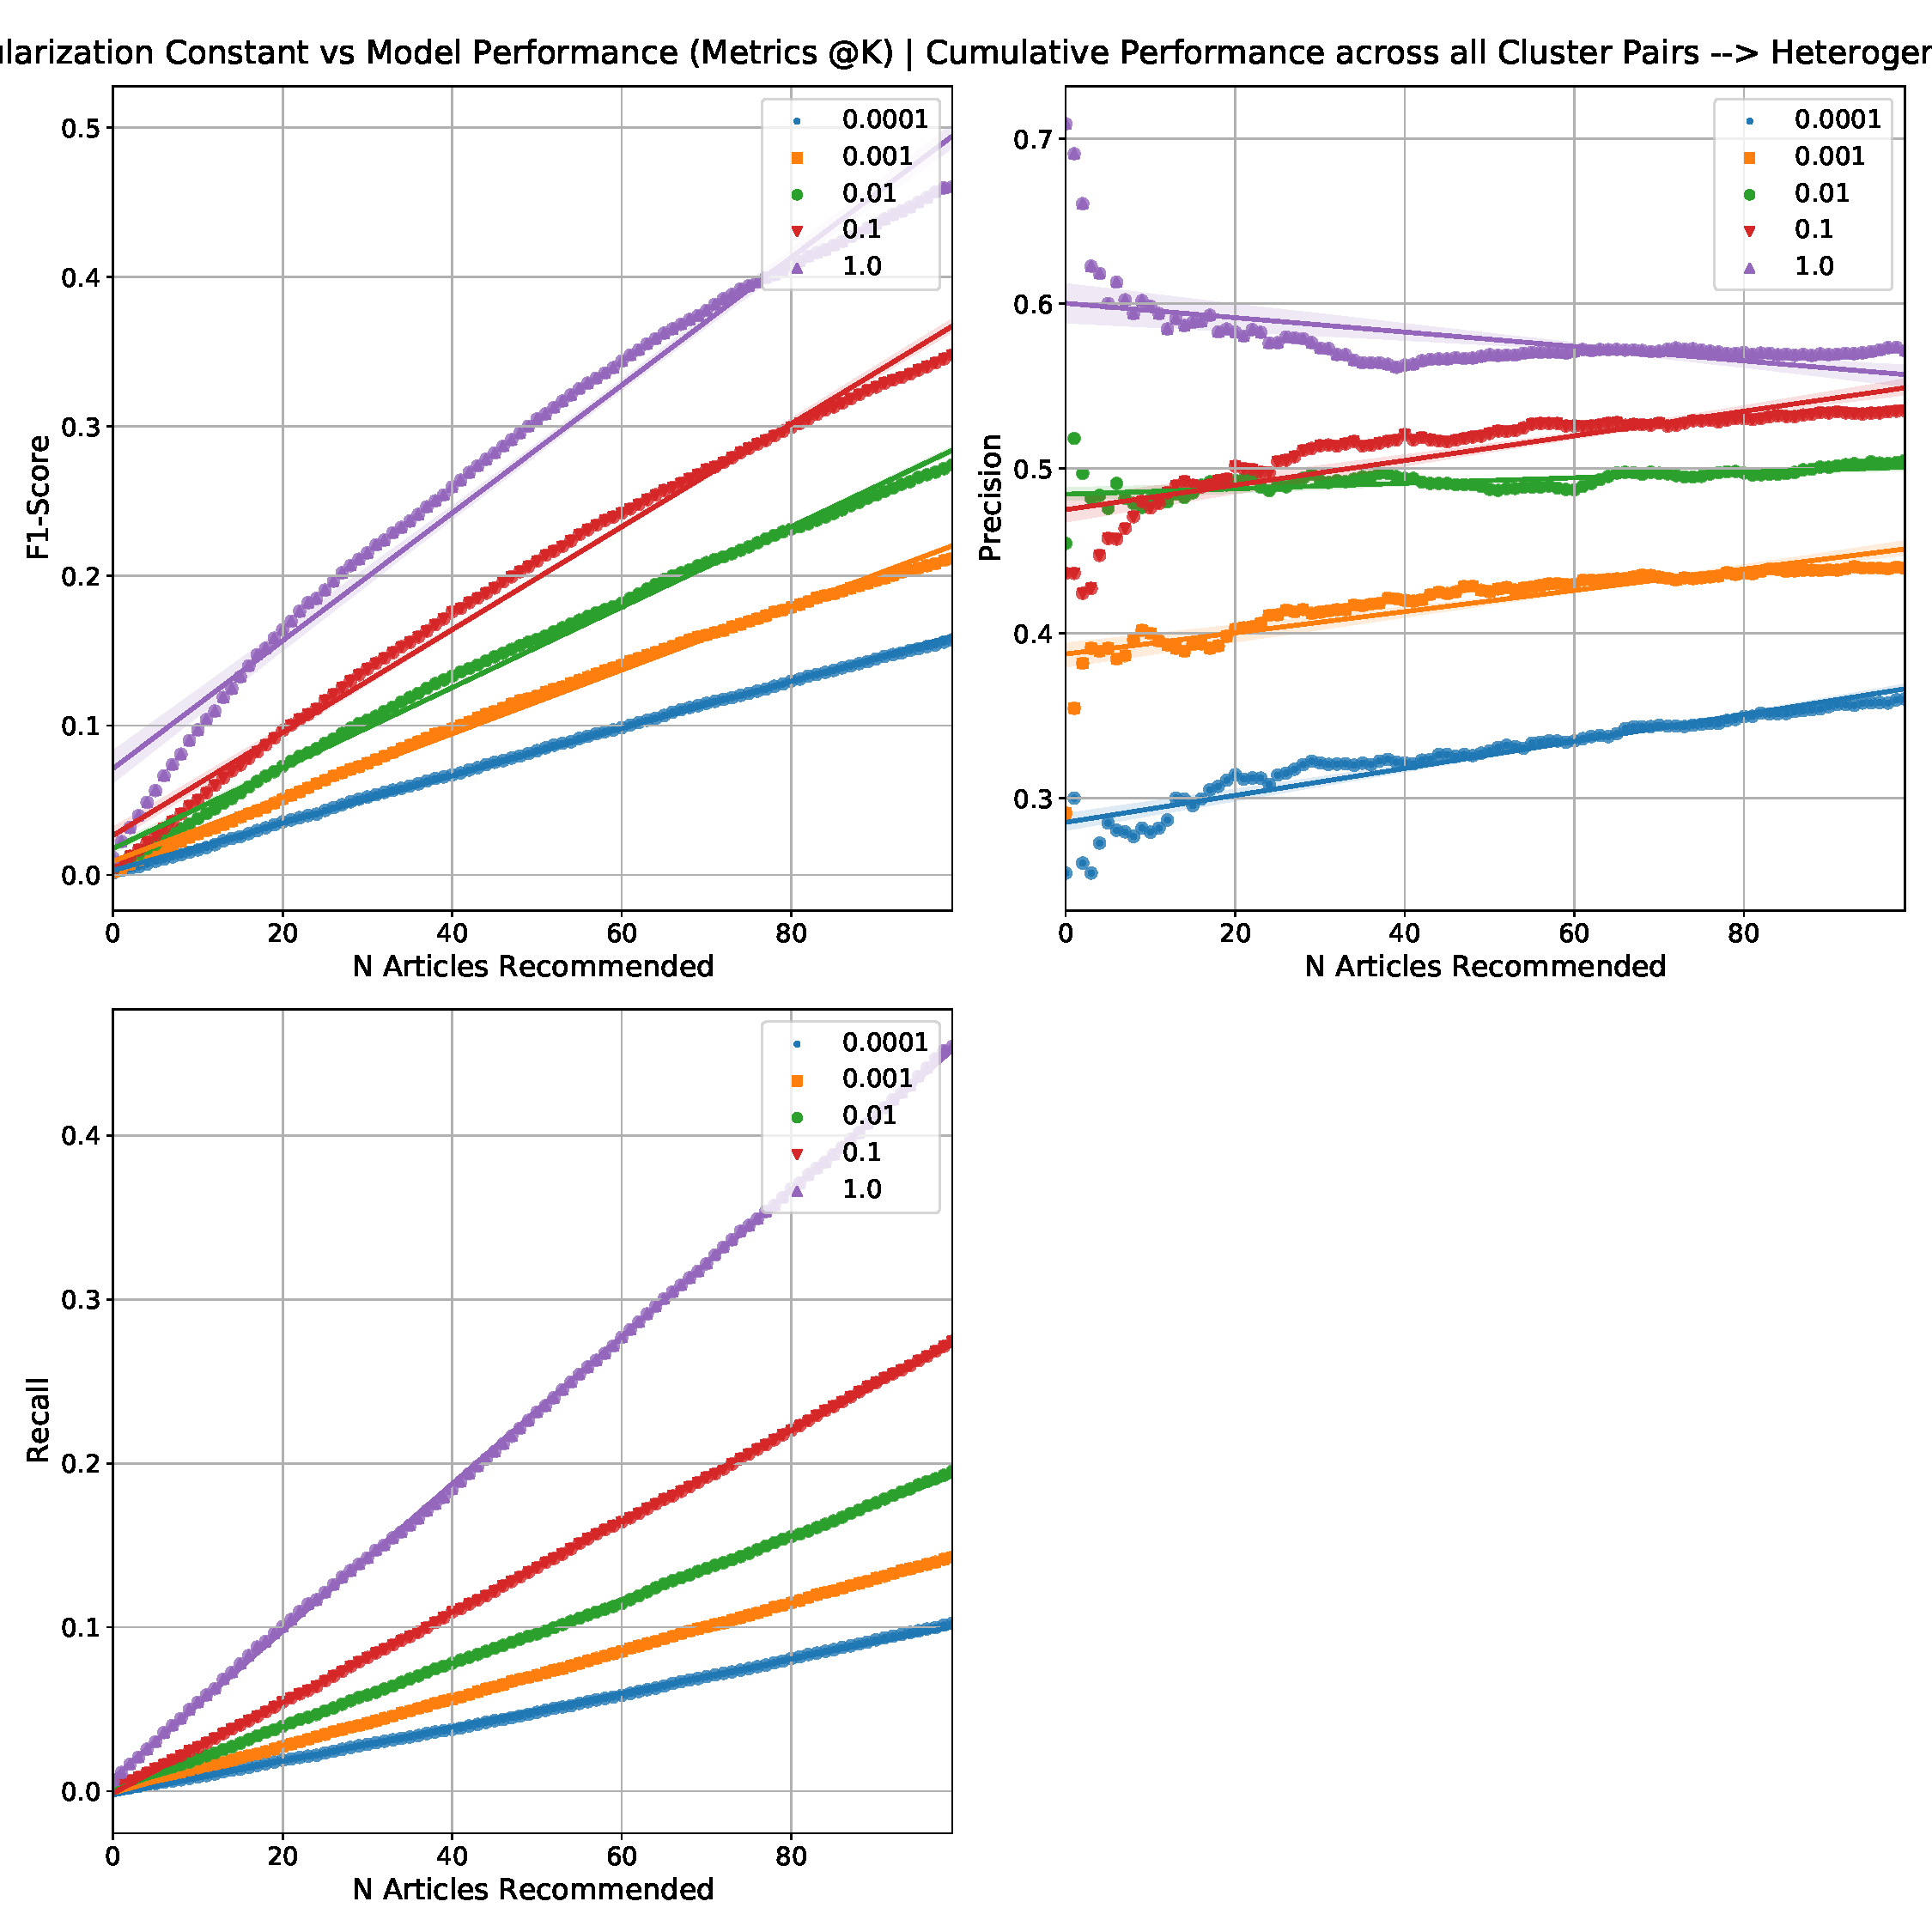
\includegraphics[width=0.8\textwidth]{Graphs/regularization_vs_model_performance_cumu_Heterogeneous.pdf}
\end{figure}



\newpage
\section{Baseline 5: Learning Rate vs Model Performance}
\begin{flushleft}
We want to measure the effect of using different learning rates to see which leads to better convergence when max-iterations are set to 1000.
\end{flushleft}
\vspace{-3ex}
\subsection{Homogeneous Users :}
\vspace{-3ex}
\begin{figure}[H]
 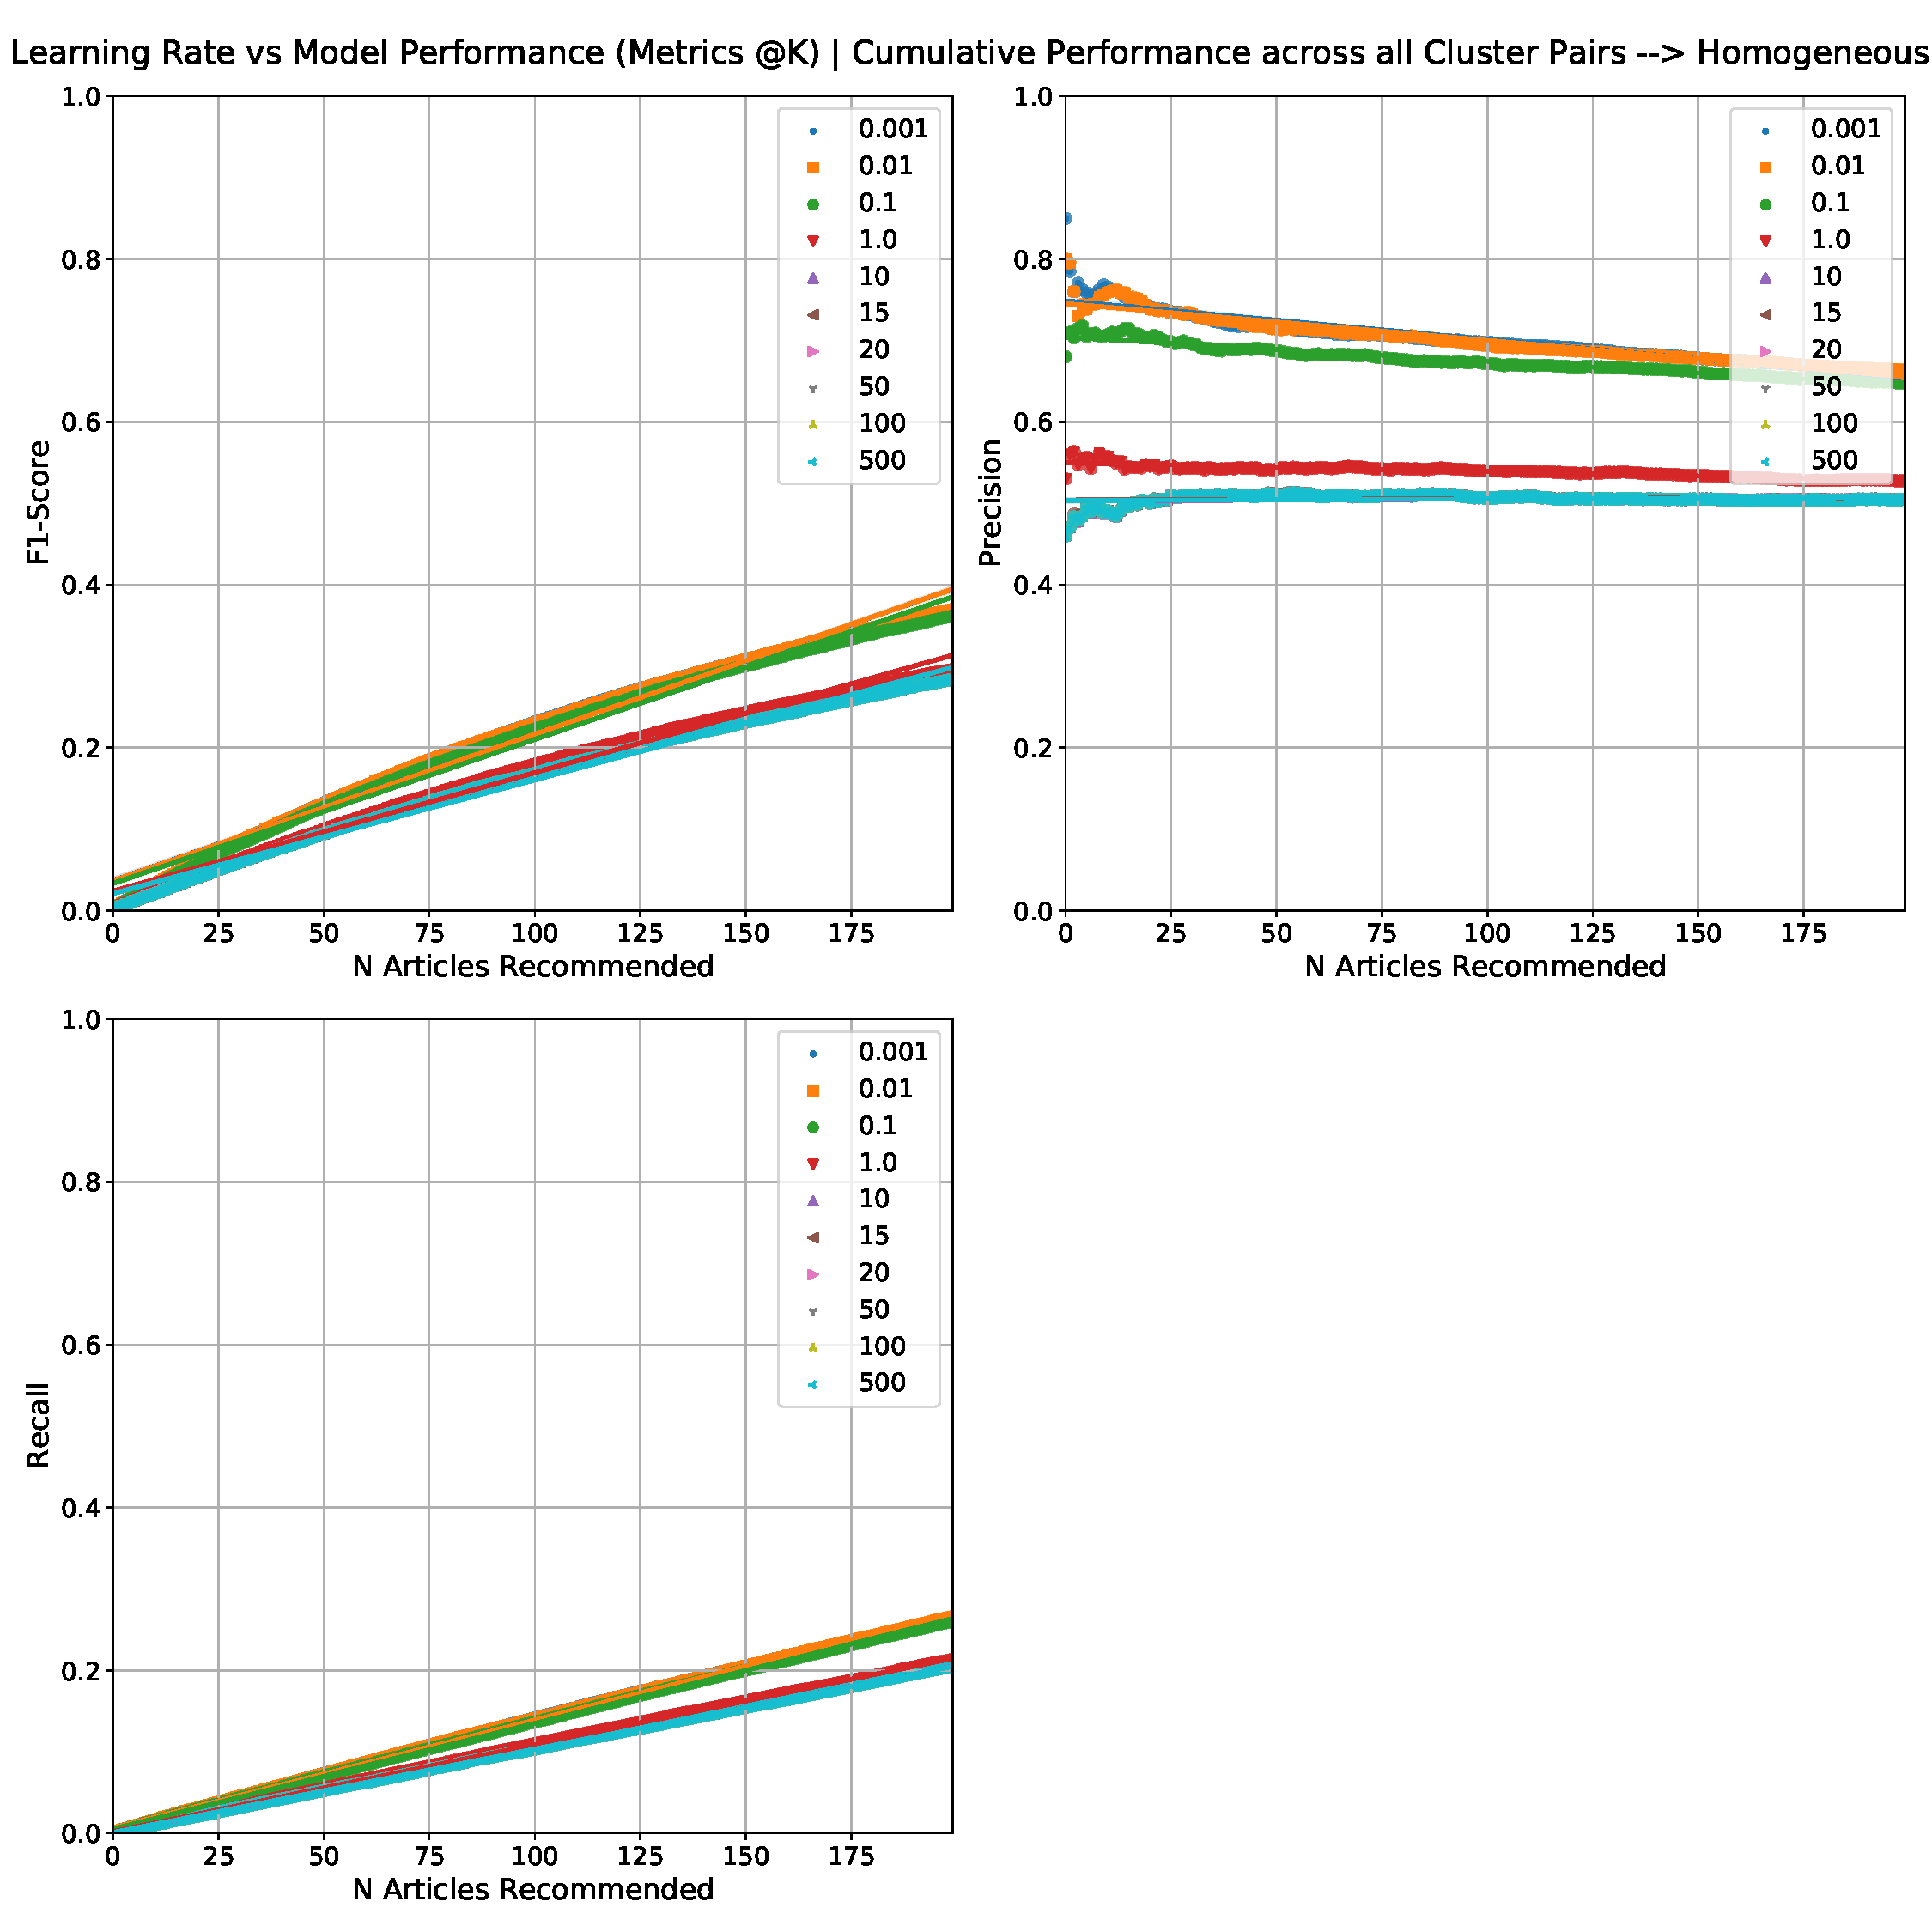
\includegraphics[width=0.8\textwidth]{Graphs/lr_vs_model_performance_cumu_Homogeneous.pdf}
\end{figure}
\subsection{Heterogeneous Users :}
\vspace{-3ex}
\begin{figure}[H]
 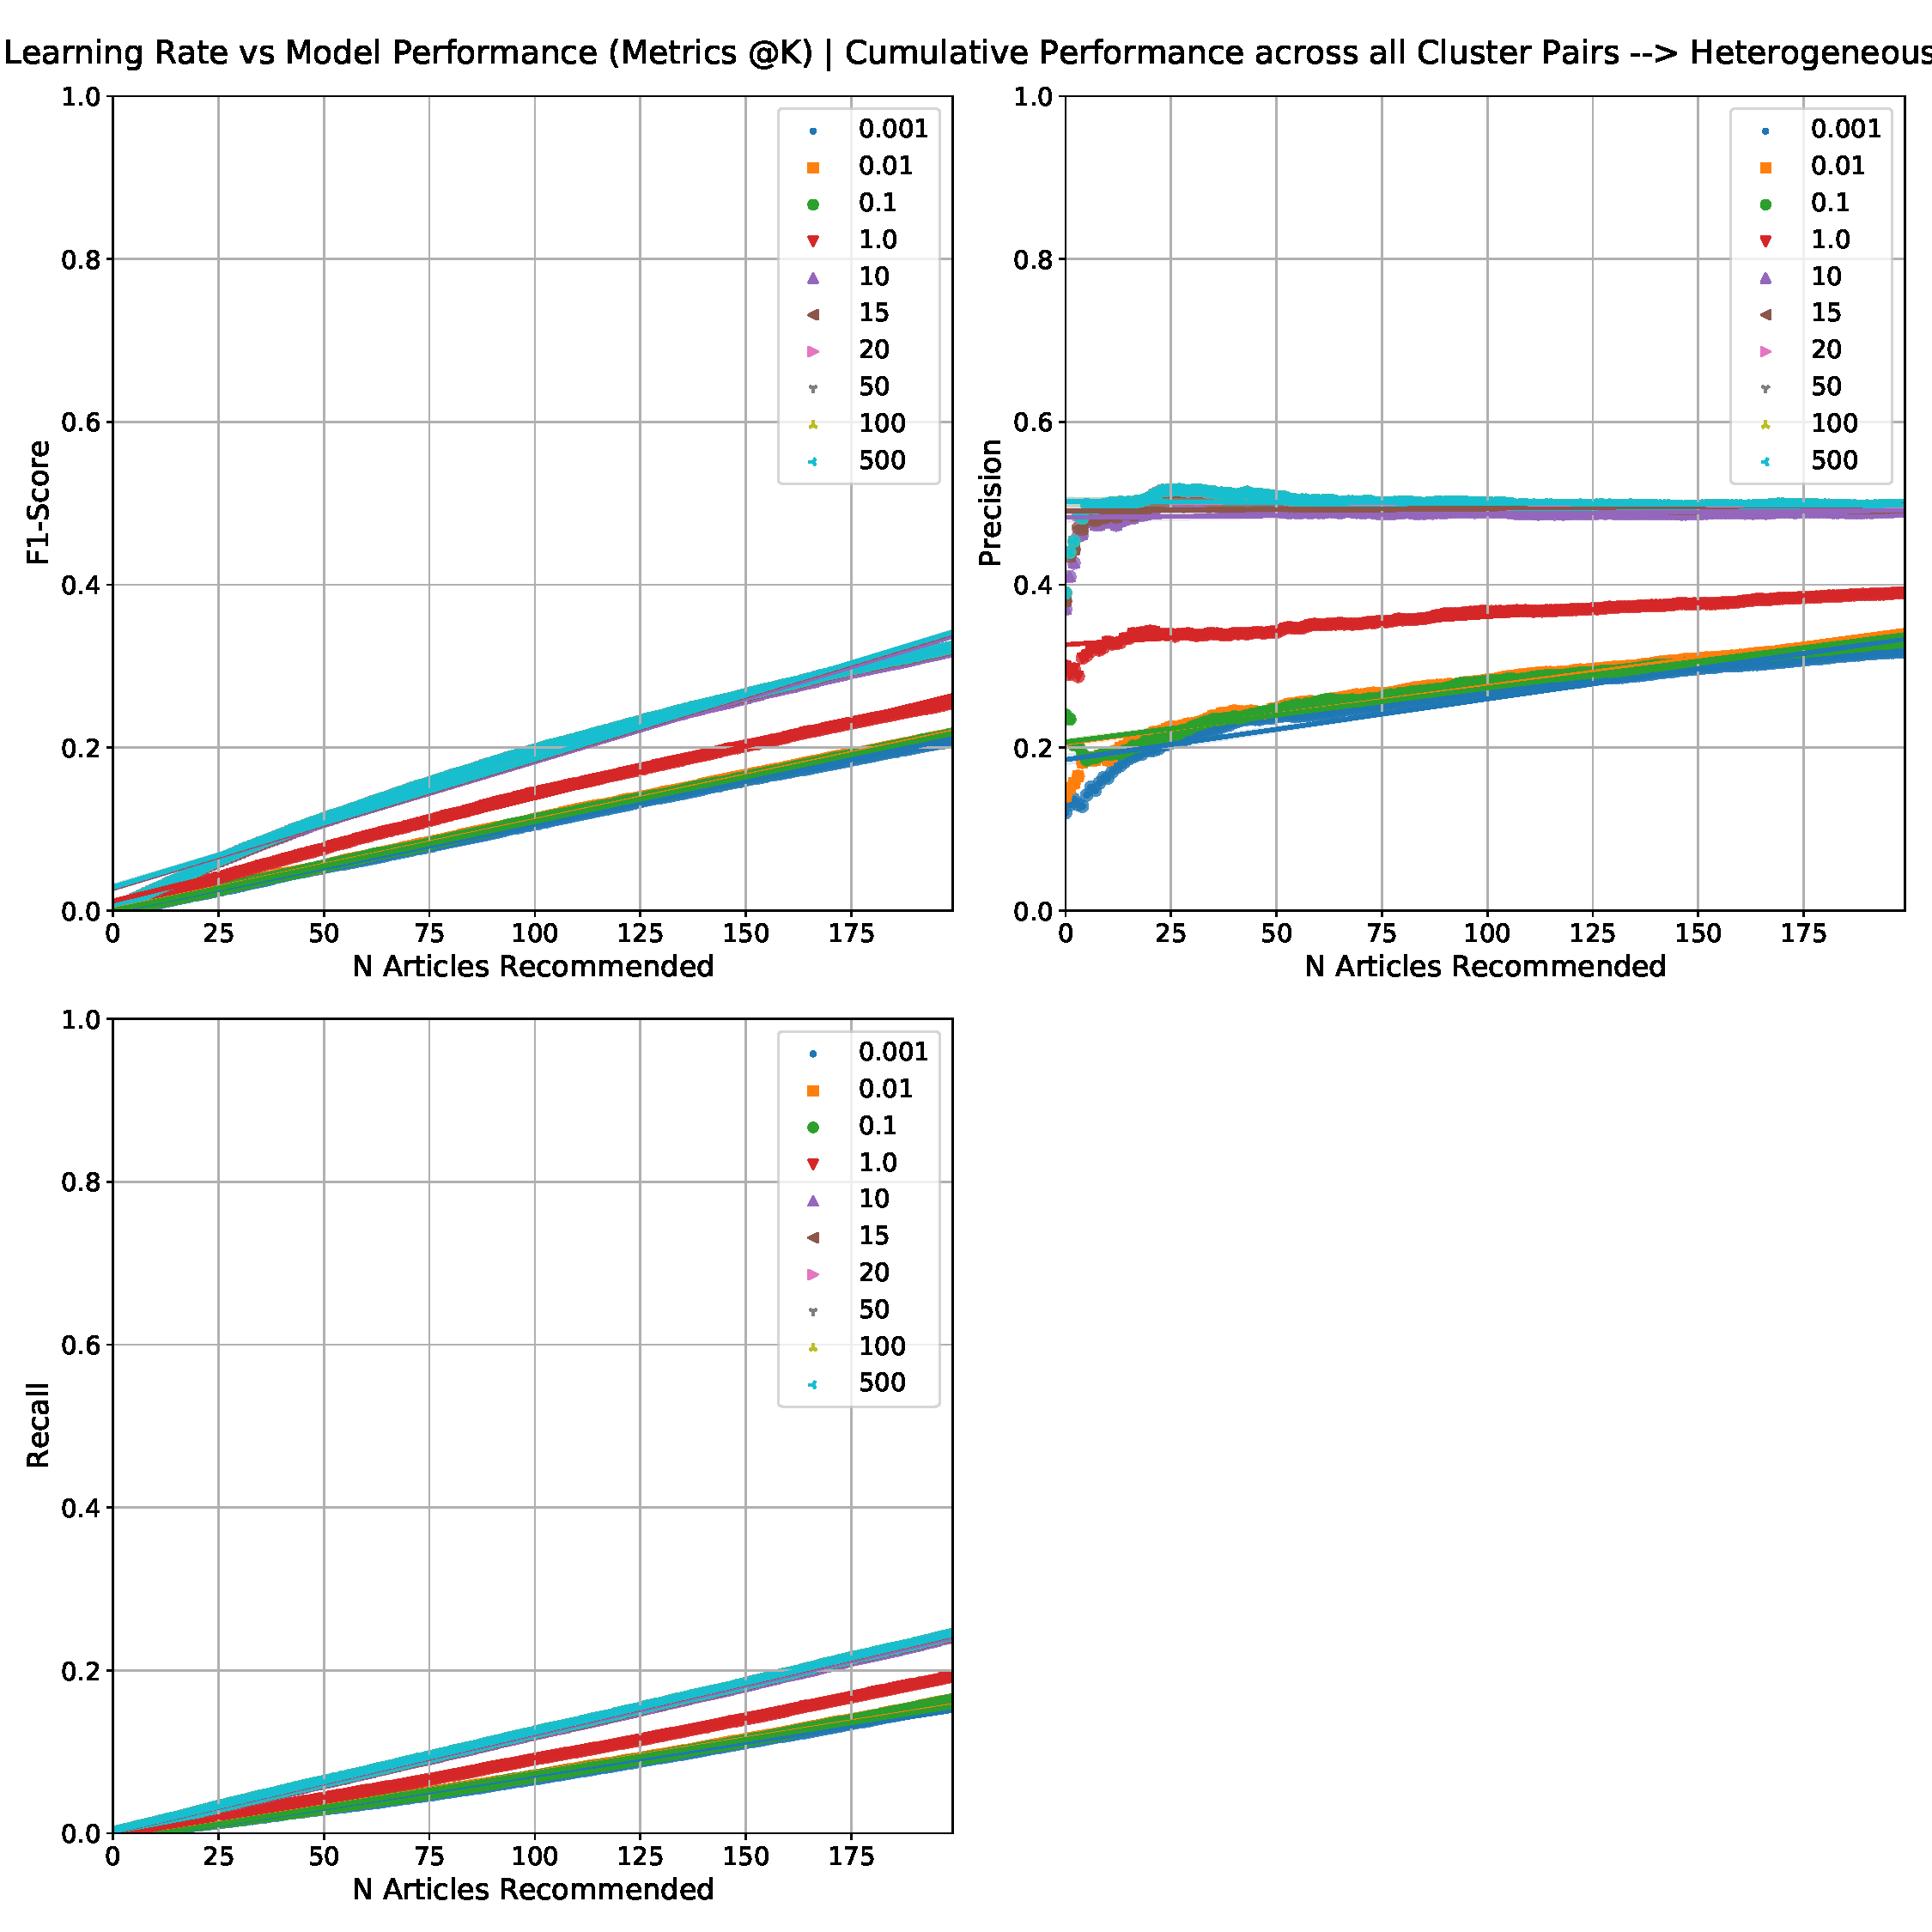
\includegraphics[width=0.8\textwidth]{Graphs/lr_vs_model_performance_cumu_Heterogeneous.pdf}
\end{figure}

\newpage
\section{Baseline 6: Model Performance on mixed Set (Cluster 1 + Cluster 2)}
\begin{flushleft}
We want to measure how well the model would perform when an article from an unseen topic arrives along with articles from the original topic the classifier was trained on
\end{flushleft}
\begin{figure}[H]
 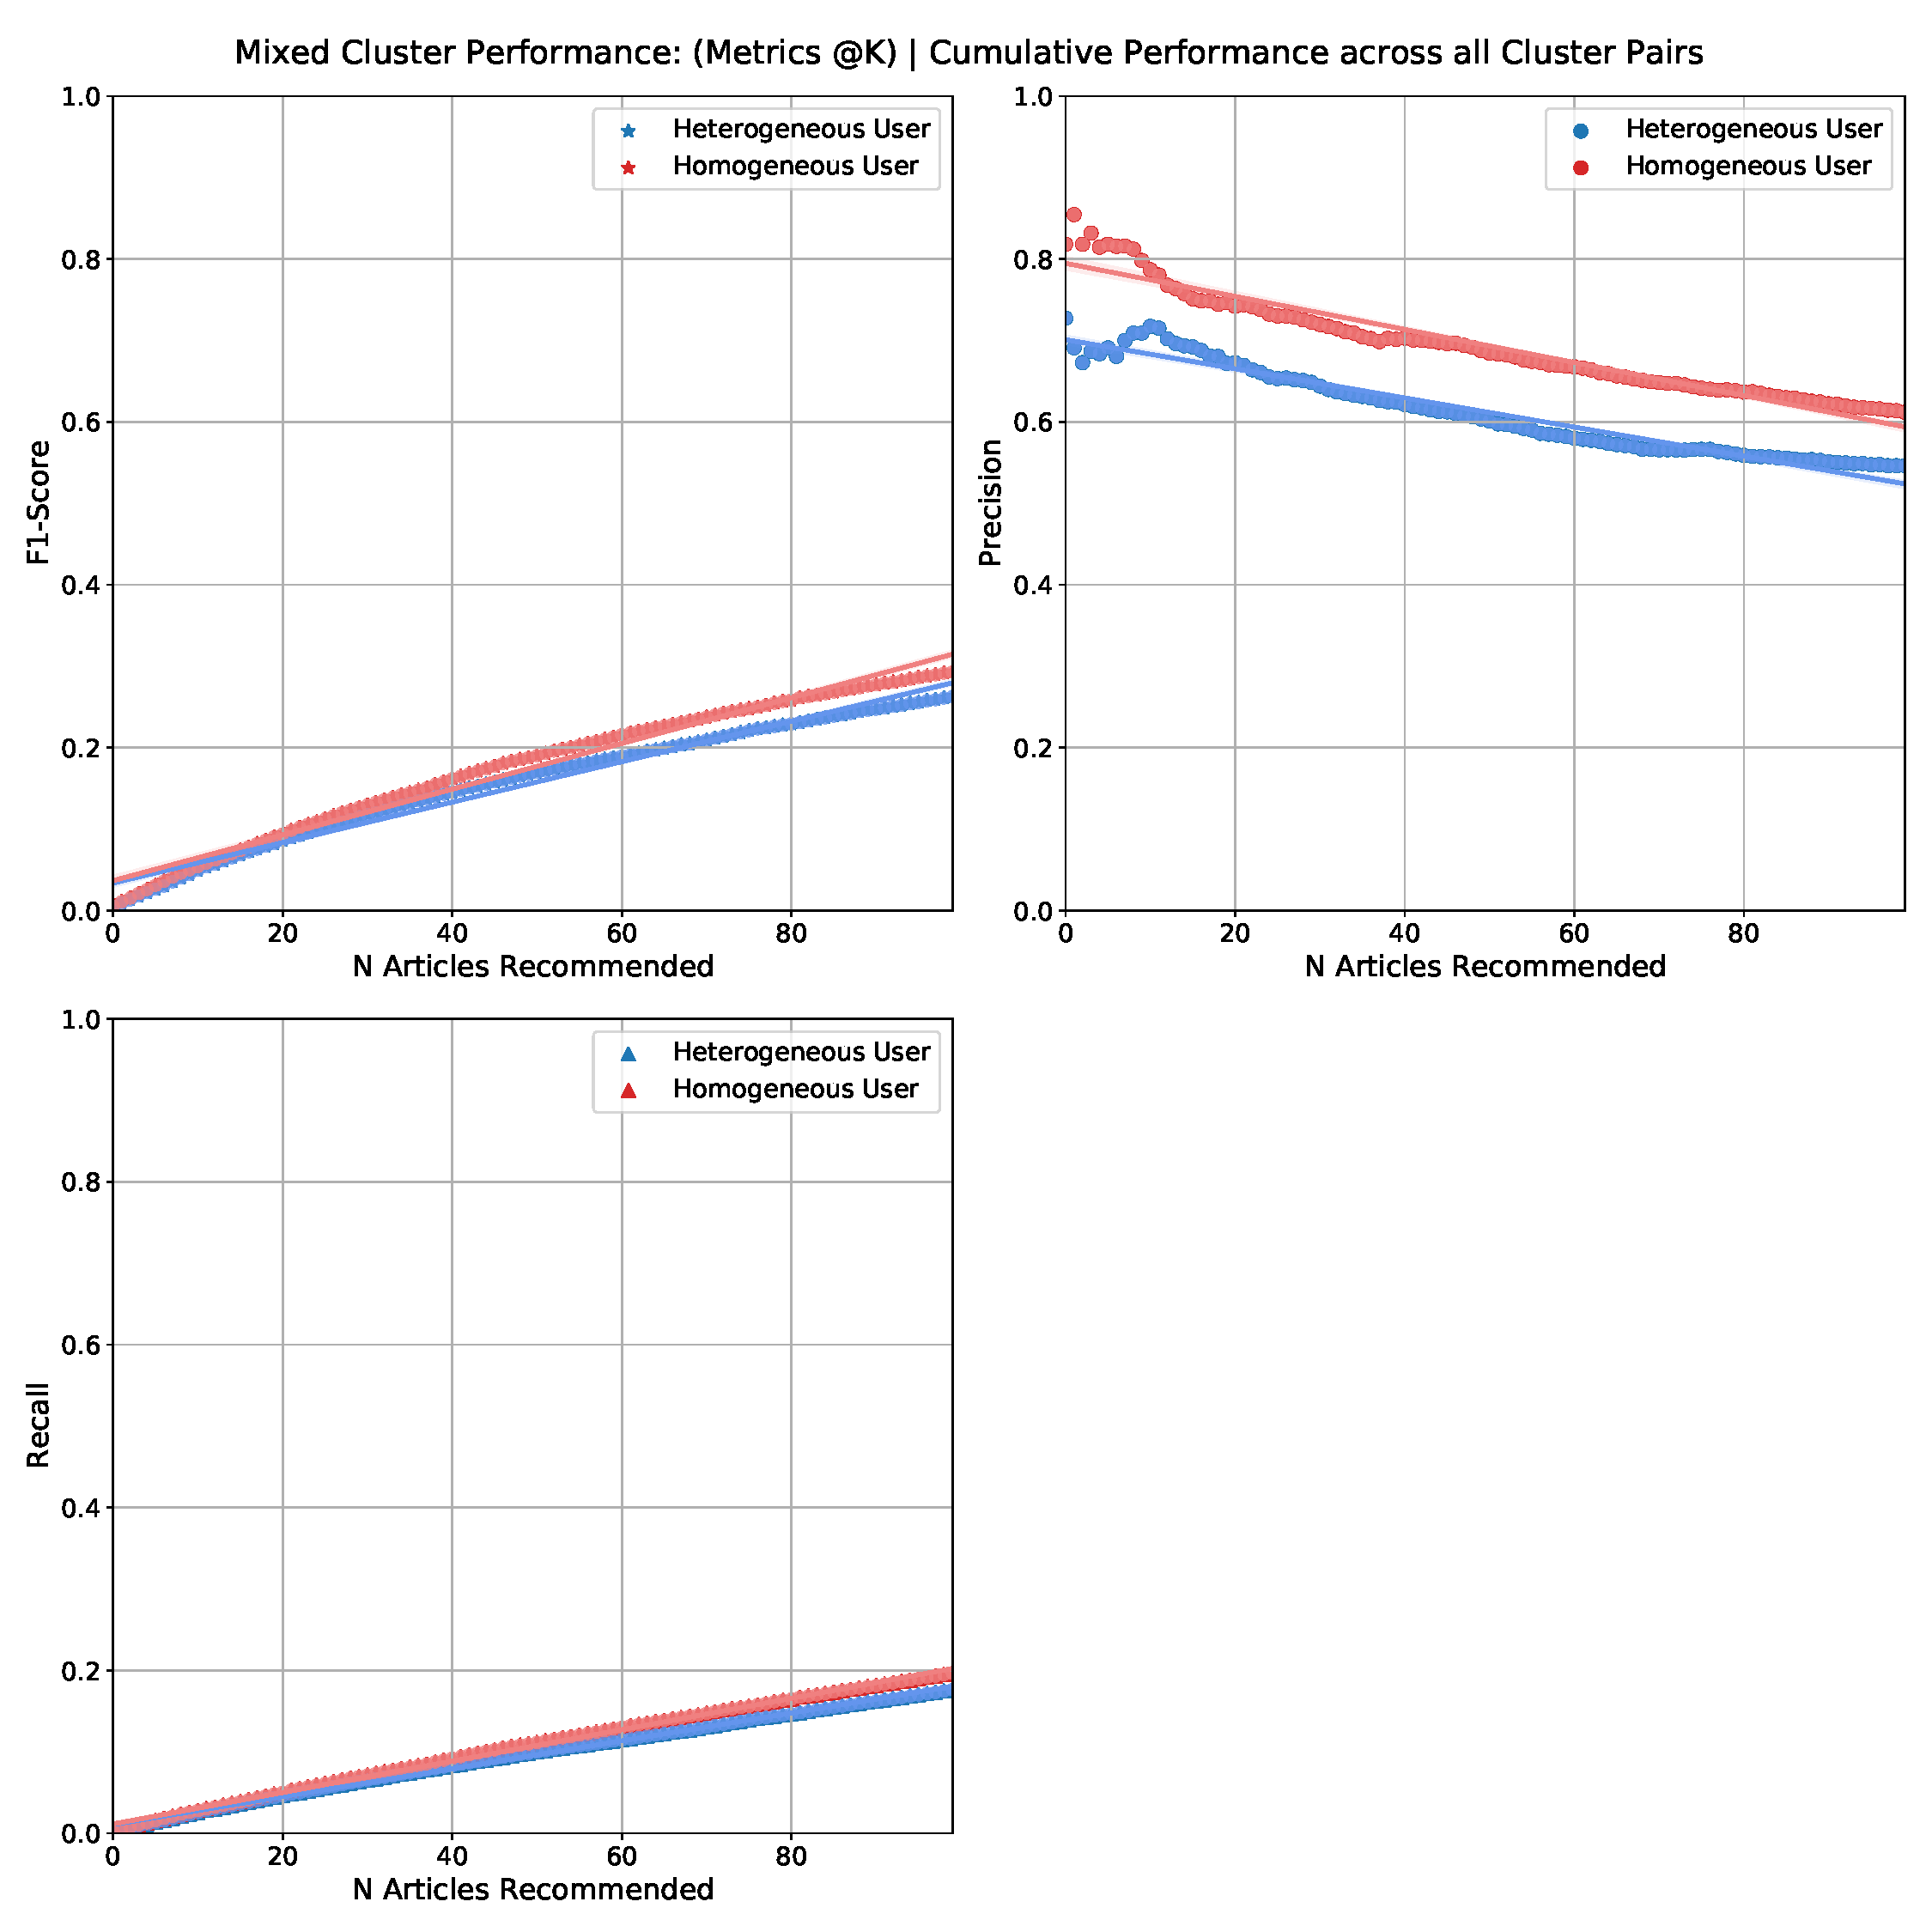
\includegraphics[width=0.8\textwidth]{Graphs/user_interaction_vs_model_performance_cumu_mixed_cluster.pdf}
\end{figure}
\begin{figure}[H]
 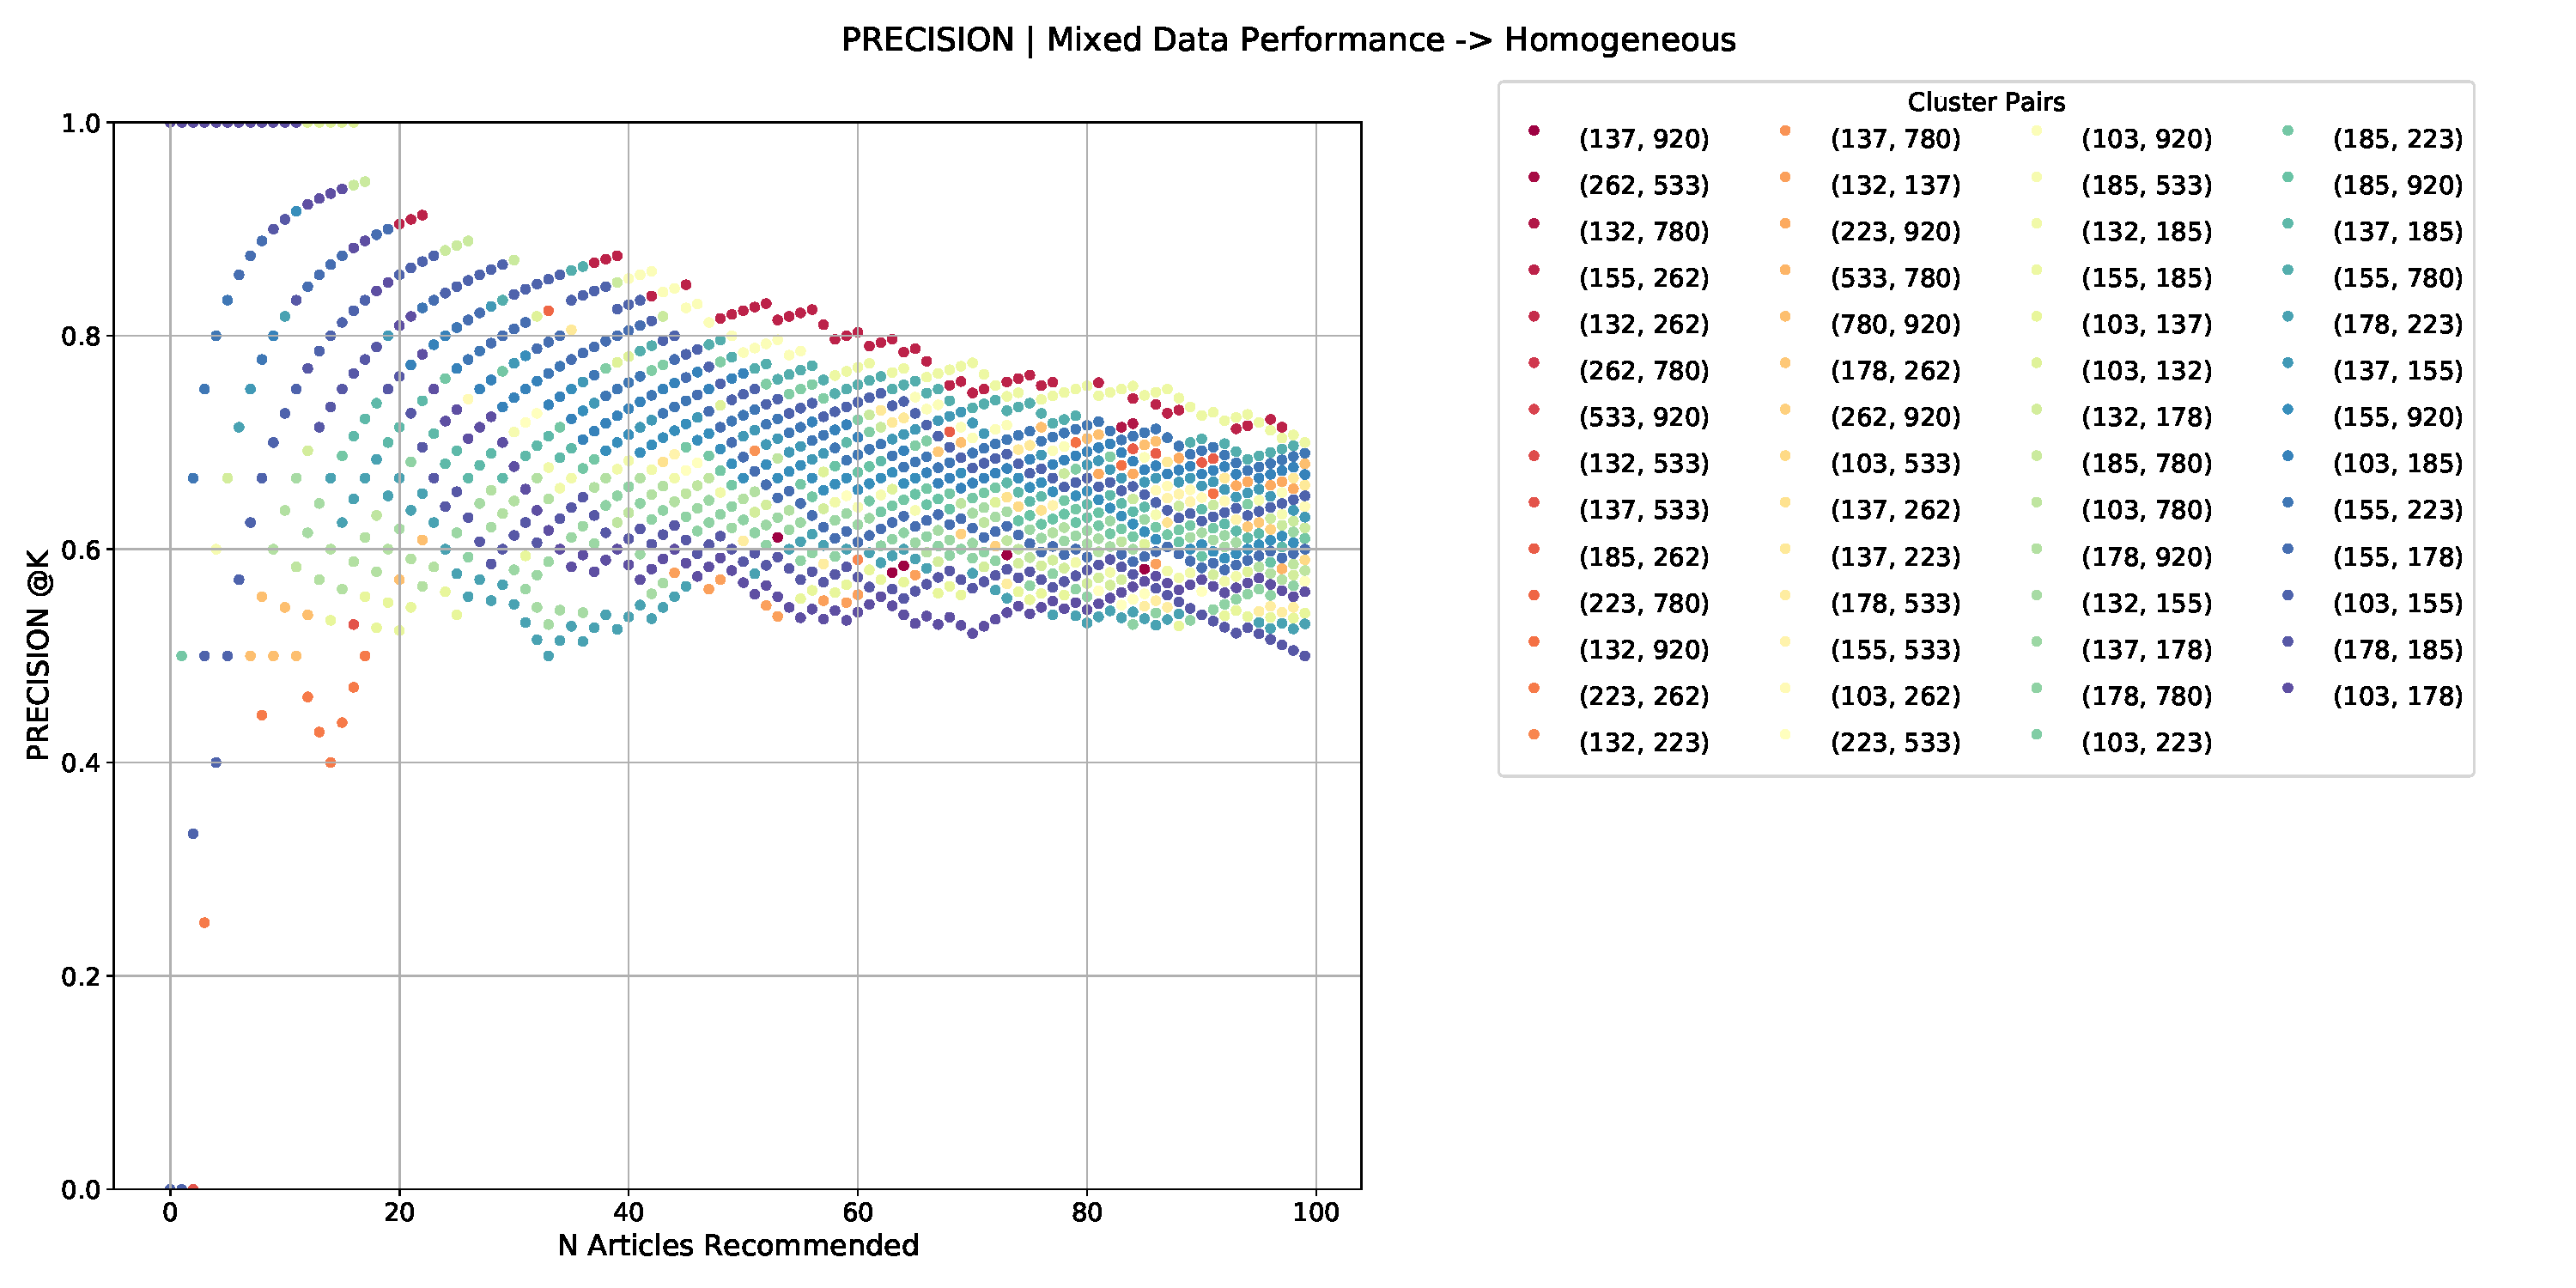
\includegraphics[width=1.0\textwidth]{Graphs/user_interaction_vs_model_performance_precision_all_cps_mixed_data_Homogeneous.pdf}
\end{figure}
\begin{figure}[H]
 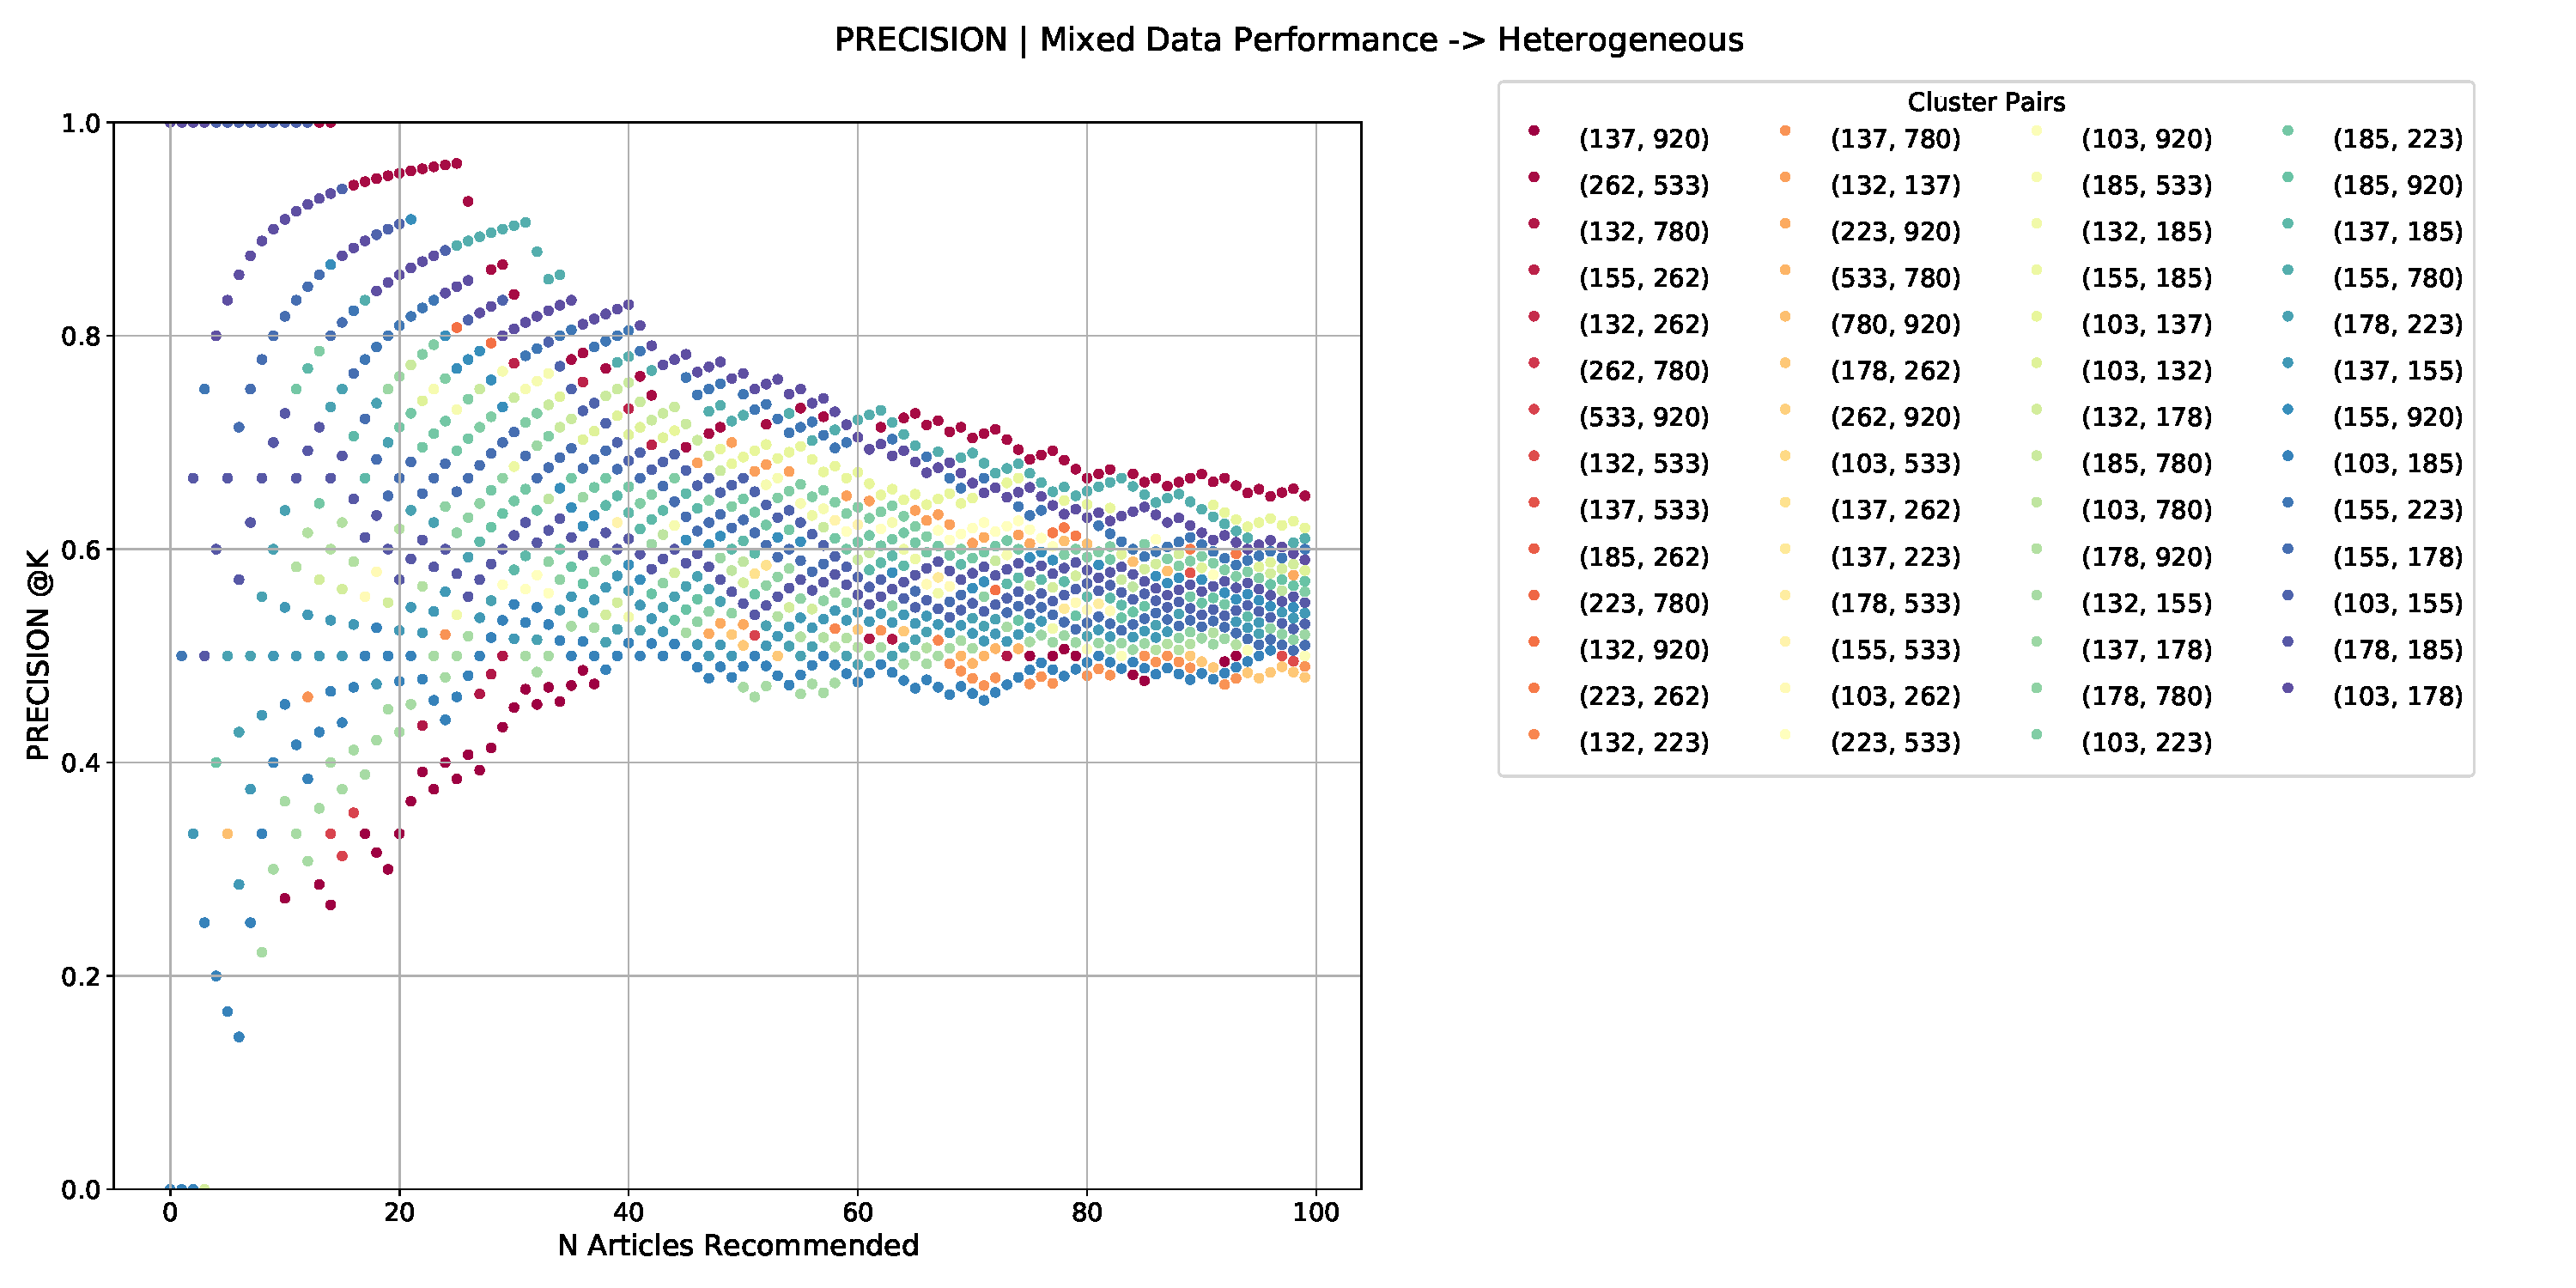
\includegraphics[width=1.0\textwidth]{Graphs/user_interaction_vs_model_performance_precision_all_cps_mixed_data_Heterogeneous.pdf}
\end{figure}

\vspace{1ex}
\section{Baseline 7: Utilizing Embedding Representations}
\begin{flushleft}
\begin{itemize}
    \item Context Independent Embeddings
    \begin{itemize}
         \item W2V : Word-2-vec Embeddings
        \item Glove Embeddings
        \item Fasttext Embeddings 
    \end{itemize}
    \item Context Dependant Embeddings
    \begin{itemize}
        \item BERT
        \item Elmo
        \item GPT (if available)
    \end{itemize}
\end{itemize}
\end{flushleft}



\end{document}